\documentclass[10pt,handout,hyperref={unicode}]{beamer}

%!TeX spellcheck = en-US,de-DE

%-------------------------------------------------------
% Beamer Theme location override
%-------------------------------------------------------

\makeatletter
  \def\beamer@calltheme#1#2#3{%
    \def\beamer@themelist{#2}
    \@for\beamer@themename:=\beamer@themelist\do%
    {\usepackage[{#1}]{\beamer@themelocation/#3\beamer@themename}}}

  \def\usefolder#1{
    \def\beamer@themelocation{#1}
  }
  \def\beamer@themelocation{}

%-------------------------------------------------------
% INCLUDE PACKAGES
%-------------------------------------------------------

\usepackage{listings} % Code listing old style
\usepackage{minted} % Code listing new style
% \usepackage{forest} % Tree graphs
\usepackage{fontspec} % UTf-8 input support
% \usepackage{multirow}
\usepackage{hyperref} % Style links
\usepackage{wasysym}
\usepackage[absolute,overlay]{textpos}
\usepackage{graphicx}
\usepackage{microtype}
\usepackage{ragged2e}
\usepackage{pgfpages}
\usepackage[ngerman]{babel}
\usepackage{docmute} % Import other .tex files ignoring document
\usepackage{multicol} % Automatically use multiple columns
\usepackage{fontawesome} % WebFonts including chref icon

%-------------------------------------------------------
% Config Theme
%-------------------------------------------------------
\usefolder{../Templates/featherZR}
\usetheme[
    progressstyle=movingCircCnt   % fixedCircCnt, movingCircCnt (moving is deault)
  ]{Feather}

  \setsansfont{HelveticaNeue}
  \setmonofont{Source Code Pro for Powerline}[Scale = MatchLowercase]

%-------------------------------------------------------
% DEFFINING AND REDEFINING COMMANDS
%-------------------------------------------------------

% \setbeameroption{show notes}
% \setbeameroption{show notes on second screen=right}

%Set Path to images
\graphicspath{{Images/}}

% colored hyperlinks
\newcommand{\chref}[2]{%
\href{#1}{{\usebeamercolor[bg]{Feather}#2} {\footnotesize\faExternalLink}}%
}

%Justification
\addtobeamertemplate{theorem begin}{}{\justifying}
\addtobeamertemplate{block begin}{}{\justifying}
\addtobeamertemplate{itemize begin}{}{\justifying}
\addtobeamertemplate{item begin}{}{\justifying}
\addtobeamertemplate{frame begin}{}{\justifying}
\addtobeamertemplate{quote begin}{}{\justifying}
\addtobeamertemplate{structure begin}{}{\justifying}

%etoolbox für nested list covering
\setbeamercovered{transparent}

%description inde
\setbeamersize{description width=0.57cm}

\makeatletter
\newcommand*\fix@beamer@close{%
  \ifnum\beamer@trivlistdepth>0
  \beamer@closeitem%
  \fi
}
\newcommand*\fix@beamer@open{%
  \ifnum\beamer@trivlistdepth>0
  \gdef\beamer@closeitem{}%
  \fi
}
\newcommand<>{\highlighton}[1]{%
  \alt#2{\structure{#1}}{{#1}}
}


\BeforeBeginEnvironment{enumerate}{\fix@beamer@close}
\AfterEndEnvironment{enumerate}{\fix@beamer@open}
\BeforeBeginEnvironment{itemize}{\fix@beamer@close}
\AfterEndEnvironment{itemize}{\fix@beamer@open}
\BeforeBeginEnvironment{description}{\fix@beamer@close}
\AfterEndEnvironment{description}{\fix@beamer@open}
\makeatother

% Codelistings
\lstset{language=PHP,
  basicstyle=\footnotesize\ttfamily,
  keywordstyle=\color{blue},
  stringstyle=\color{red},
  commentstyle=\color{gray},
  breaklines=true,
  tabsize=2
}

% Codelistings
\definecolor{monokaibg}{HTML}{002833}
\definecolor{highlightbg}{HTML}{004550}

\setminted{
  autogobble=true,
  bgcolor=monokaibg,
  breaklines=true,
  fontsize=\footnotesize,
  highlightcolor=highlightbg,
  linenos=true,
  labelposition=bottomline,
  rulecolor=white,
  style=native,
}

\setmintedinline{
  bgcolor={},
  fontsize=\normalsize,
  style=manni
}

%-------------------------------------------------------
% INFORMATION IN THE TITLE PAGE
%-------------------------------------------------------

\title[Unit Tests ] % [] is optional - is placed on the bottom of the sidebar on every slide
{ % is placed on the title page
      \textbf{Unit Tests}
}

\subtitle[ -- Testen mit Hilfe von Unit Tests]
{
%      \textbf{v. 1.0.0}
}

\author[Sebastian Knott]{Sebastian Knott}

\institute[]
{
      ZooRoyal IT\\

  %there must be an empty line above this line - otherwise some unwanted space is added between the university and the country (I do not know why;( )
}

\date{\today}

%-------------------------------------------------------
% THE TITLE OF THE PRESENTATION
%-------------------------------------------------------

\begin{document}

\documentclass[10pt,hyperref={unicode}]{beamer}

%!TeX spellcheck = en-US,de-DE

%-------------------------------------------------------
% Beamer Theme location override
%-------------------------------------------------------

\makeatletter
  \def\beamer@calltheme#1#2#3{%
    \def\beamer@themelist{#2}
    \@for\beamer@themename:=\beamer@themelist\do%
    {\usepackage[{#1}]{\beamer@themelocation/#3\beamer@themename}}}

  \def\usefolder#1{
    \def\beamer@themelocation{#1}
  }
  \def\beamer@themelocation{}

%-------------------------------------------------------
% INCLUDE PACKAGES
%-------------------------------------------------------

\usepackage{listings} % Code listing old style
\usepackage{minted} % Code listing new style
% \usepackage{forest} % Tree graphs
\usepackage{fontspec} % UTf-8 input support
% \usepackage{multirow}
\usepackage{hyperref} % Style links
\usepackage{wasysym}
\usepackage[absolute,overlay]{textpos}
\usepackage{graphicx}
\usepackage{microtype}
\usepackage{ragged2e}
\usepackage{pgfpages}
\usepackage[ngerman]{babel}
\usepackage{docmute} % Import other .tex files ignoring document
\usepackage{multicol} % Automatically use multiple columns
\usepackage{fontawesome} % WebFonts including chref icon

%-------------------------------------------------------
% Config Theme
%-------------------------------------------------------
\usefolder{../Templates/featherZR}
\usetheme[
    progressstyle=movingCircCnt   % fixedCircCnt, movingCircCnt (moving is deault)
  ]{Feather}

  \setsansfont{HelveticaNeue}
  \setmonofont{Source Code Pro for Powerline}[Scale = MatchLowercase]

%-------------------------------------------------------
% DEFFINING AND REDEFINING COMMANDS
%-------------------------------------------------------

% \setbeameroption{show notes}
% \setbeameroption{show notes on second screen=right}

%Set Path to images
\graphicspath{{Images/}}

% colored hyperlinks
\newcommand{\chref}[2]{%
\href{#1}{{\usebeamercolor[bg]{Feather}#2} {\footnotesize\faExternalLink}}%
}

%Justification
\addtobeamertemplate{theorem begin}{}{\justifying}
\addtobeamertemplate{block begin}{}{\justifying}
\addtobeamertemplate{itemize begin}{}{\justifying}
\addtobeamertemplate{item begin}{}{\justifying}
\addtobeamertemplate{frame begin}{}{\justifying}
\addtobeamertemplate{quote begin}{}{\justifying}
\addtobeamertemplate{structure begin}{}{\justifying}

%etoolbox für nested list covering
\setbeamercovered{transparent}

%description inde
\setbeamersize{description width=0.57cm}

\makeatletter
\newcommand*\fix@beamer@close{%
  \ifnum\beamer@trivlistdepth>0
  \beamer@closeitem%
  \fi
}
\newcommand*\fix@beamer@open{%
  \ifnum\beamer@trivlistdepth>0
  \gdef\beamer@closeitem{}%
  \fi
}
\newcommand<>{\highlighton}[1]{%
  \alt#2{\structure{#1}}{{#1}}
}


\BeforeBeginEnvironment{enumerate}{\fix@beamer@close}
\AfterEndEnvironment{enumerate}{\fix@beamer@open}
\BeforeBeginEnvironment{itemize}{\fix@beamer@close}
\AfterEndEnvironment{itemize}{\fix@beamer@open}
\BeforeBeginEnvironment{description}{\fix@beamer@close}
\AfterEndEnvironment{description}{\fix@beamer@open}
\makeatother

% Codelistings
\lstset{language=PHP,
  basicstyle=\footnotesize\ttfamily,
  keywordstyle=\color{blue},
  stringstyle=\color{red},
  commentstyle=\color{gray},
  breaklines=true,
  tabsize=2
}

% Codelistings
\definecolor{monokaibg}{HTML}{002833}
\definecolor{highlightbg}{HTML}{004550}

\setminted{
  autogobble=true,
  bgcolor=monokaibg,
  breaklines=true,
  fontsize=\footnotesize,
  highlightcolor=highlightbg,
  linenos=true,
  labelposition=bottomline,
  rulecolor=white,
  style=native,
}

\setmintedinline{
  bgcolor={},
  fontsize=\normalsize,
  style=manni
}

%-------------------------------------------------------
% INFORMATION IN THE TITLE PAGE
%-------------------------------------------------------

\title[Unit Tests ] % [] is optional - is placed on the bottom of the sidebar on every slide
{ % is placed on the title page
      \textbf{Unit Tests}
}

\subtitle[ -- Testen mit Hilfe von Unit Tests]
{
%      \textbf{v. 1.0.0}
}

\author[Sebastian Knott]{Sebastian Knott}

\institute[]
{
      ZooRoyal IT\\

  %there must be an empty line above this line - otherwise some unwanted space is added between the university and the country (I do not know why;( )
}

\date{\today}

%-------------------------------------------------------
% THE TITLE OF THE PRESENTATION
%-------------------------------------------------------

\begin{document}

{\1
\begin{frame}[plain,noframenumbering] % the plain option removes the header from the title page, noframenumbering removes the numbering of this frame only
  \titlepage% call the title page information from above
\end{frame}}

% \AtBeginSection[]
% {
%   \frame<handout:0>
%   {
%     \frametitle{Überblick}
%     \tableofcontents[currentsection,hideothersubsections,sectionstyle=show/shaded,subsectionstyle=show/shaded]
%   }
% }

\AtBeginSubsection[]
{
  \frame<handout:0>
  {
    \frametitle{Überblick}
    \tableofcontents[currentsection,hideothersubsections,sectionstyle=show/shaded,subsectionstyle=show/shaded]
  }
}

\AtBeginSubsubsection[]
{
  \frame<handout:0>
  {
    \frametitle{Überblick}
    \tableofcontents[currentsection,hideothersubsections,sectionstyle=show/shaded,subsectionstyle=show/shaded,subsubsectionstyle=show/shaded]
  }
}

%-------------------------------------------------------
% THE BODY OF THE PRESENTATION
%-------------------------------------------------------

\begin{frame}
  \frametitle{Überblick}
  \tableofcontents[currentsection,sectionstyle=show,subsectionstyle=show,subsubsectionstyle=hide]
\end{frame}


\section{Grundlagen}


\subsection{Einordnung}


\begin{frame}
  \frametitle{Einordnung}
  \framesubtitle{Übersicht Fehlerbehandlung}
  \begin{figure}
    \begin{center}
      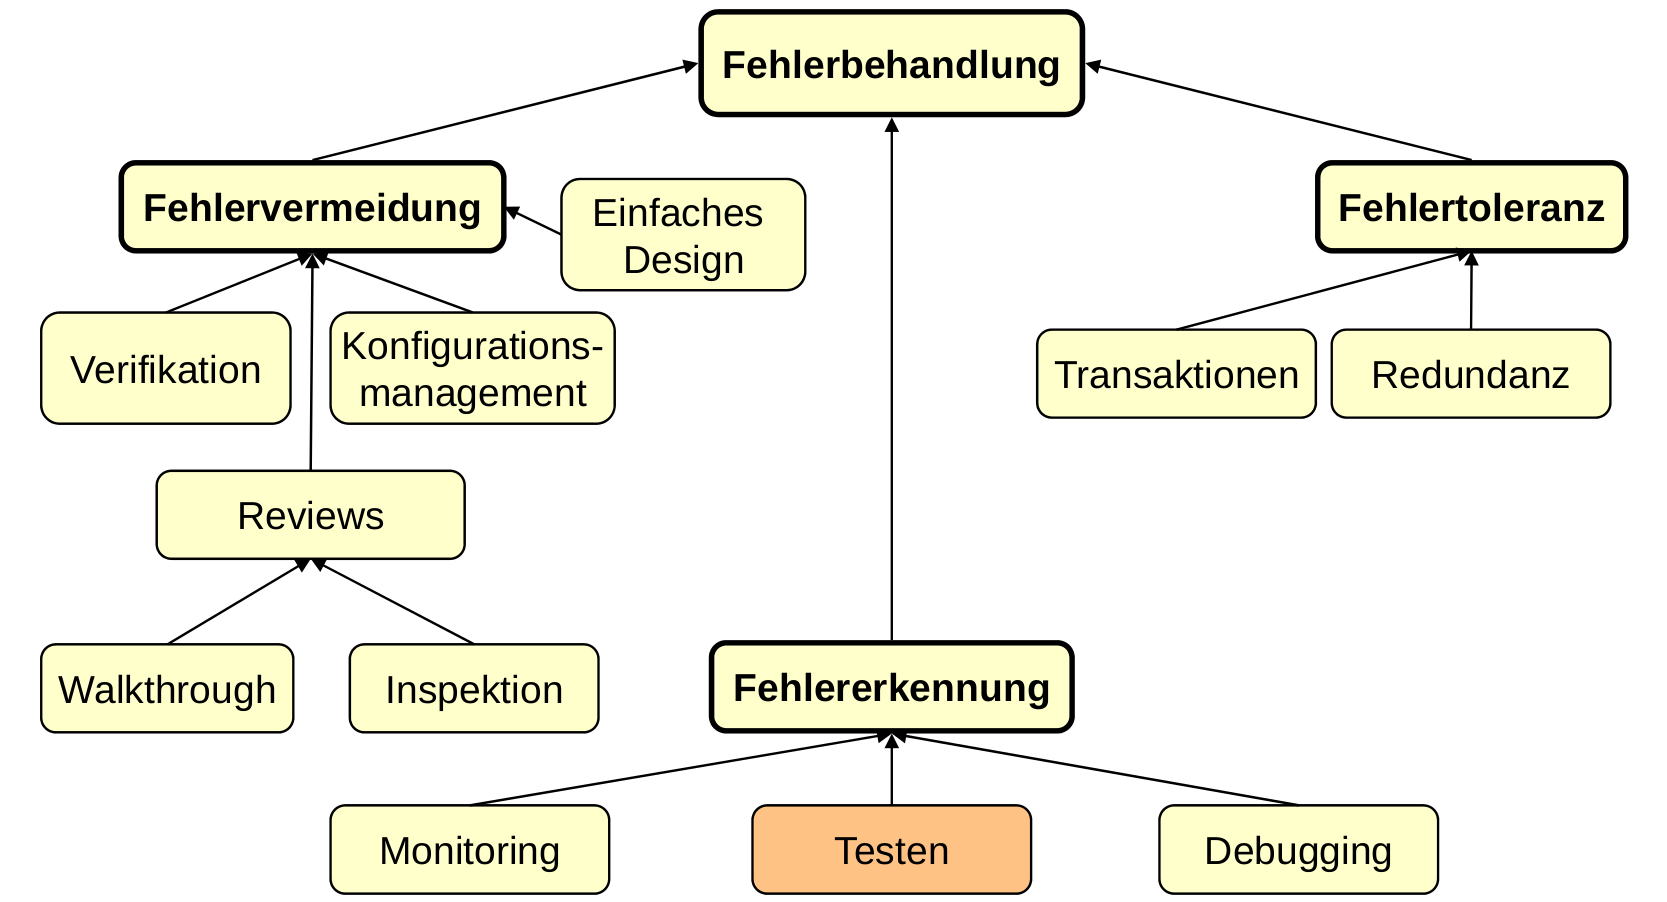
\includegraphics[width=\textwidth]{uebersicht-1}
    \end{center}
  \end{figure}
\end{frame}


\begin{frame}
  \frametitle{Einordnung}
  \framesubtitle{Übersicht Fehlererkennung}
  \begin{figure}
    \begin{center}
      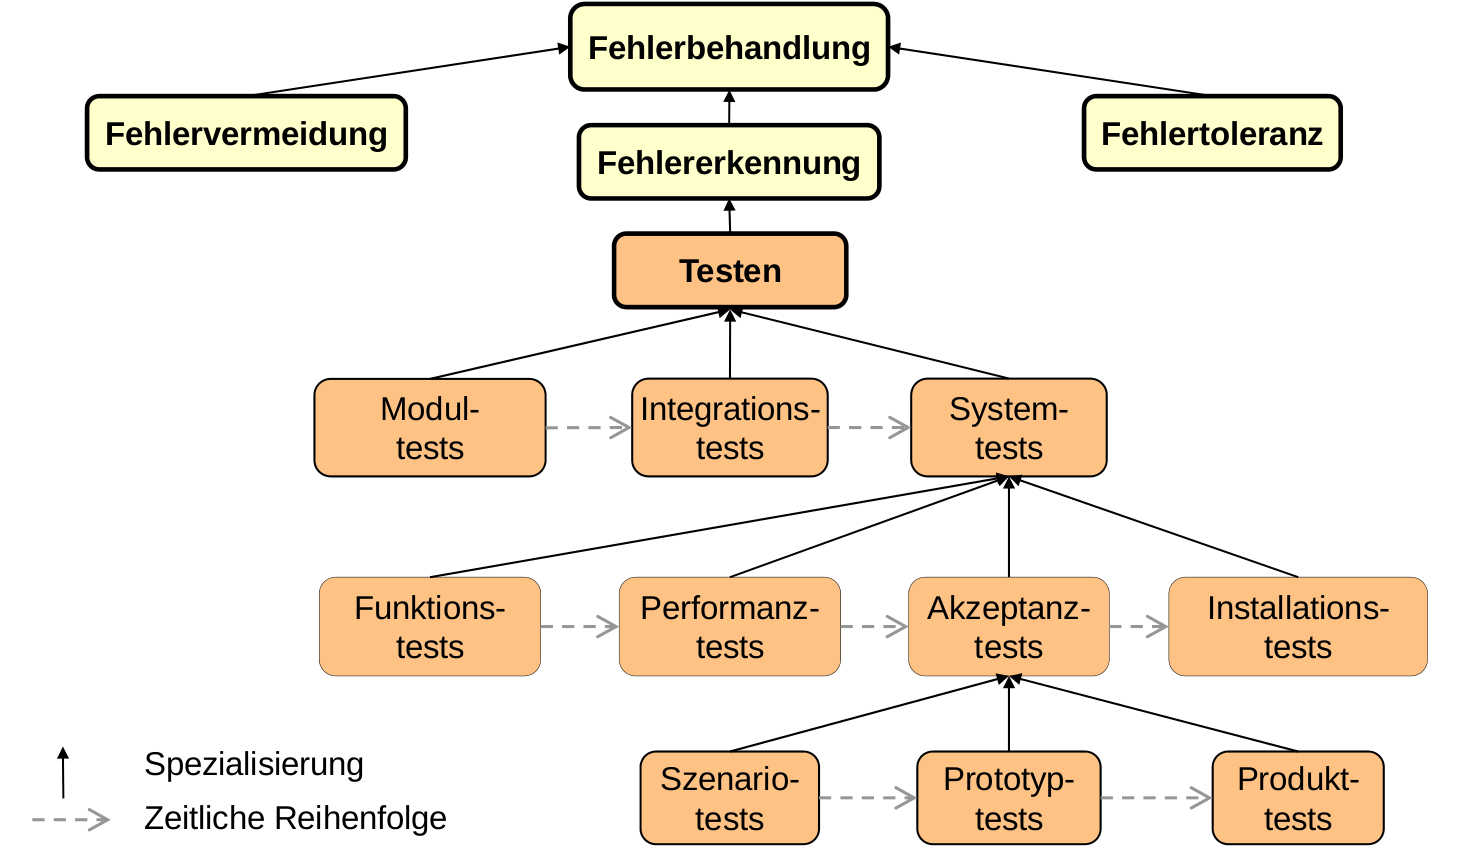
\includegraphics[width=\textwidth]{uebersicht-2}
    \end{center}
  \end{figure}
\end{frame}


\subsection{Lebenszyklus Tests}


\begin{frame}
  \frametitle{Lebenszyklus Tests}
  \framesubtitle{\dots in 9 Schritten oder weniger}
  \begin{figure}
    \begin{center}
      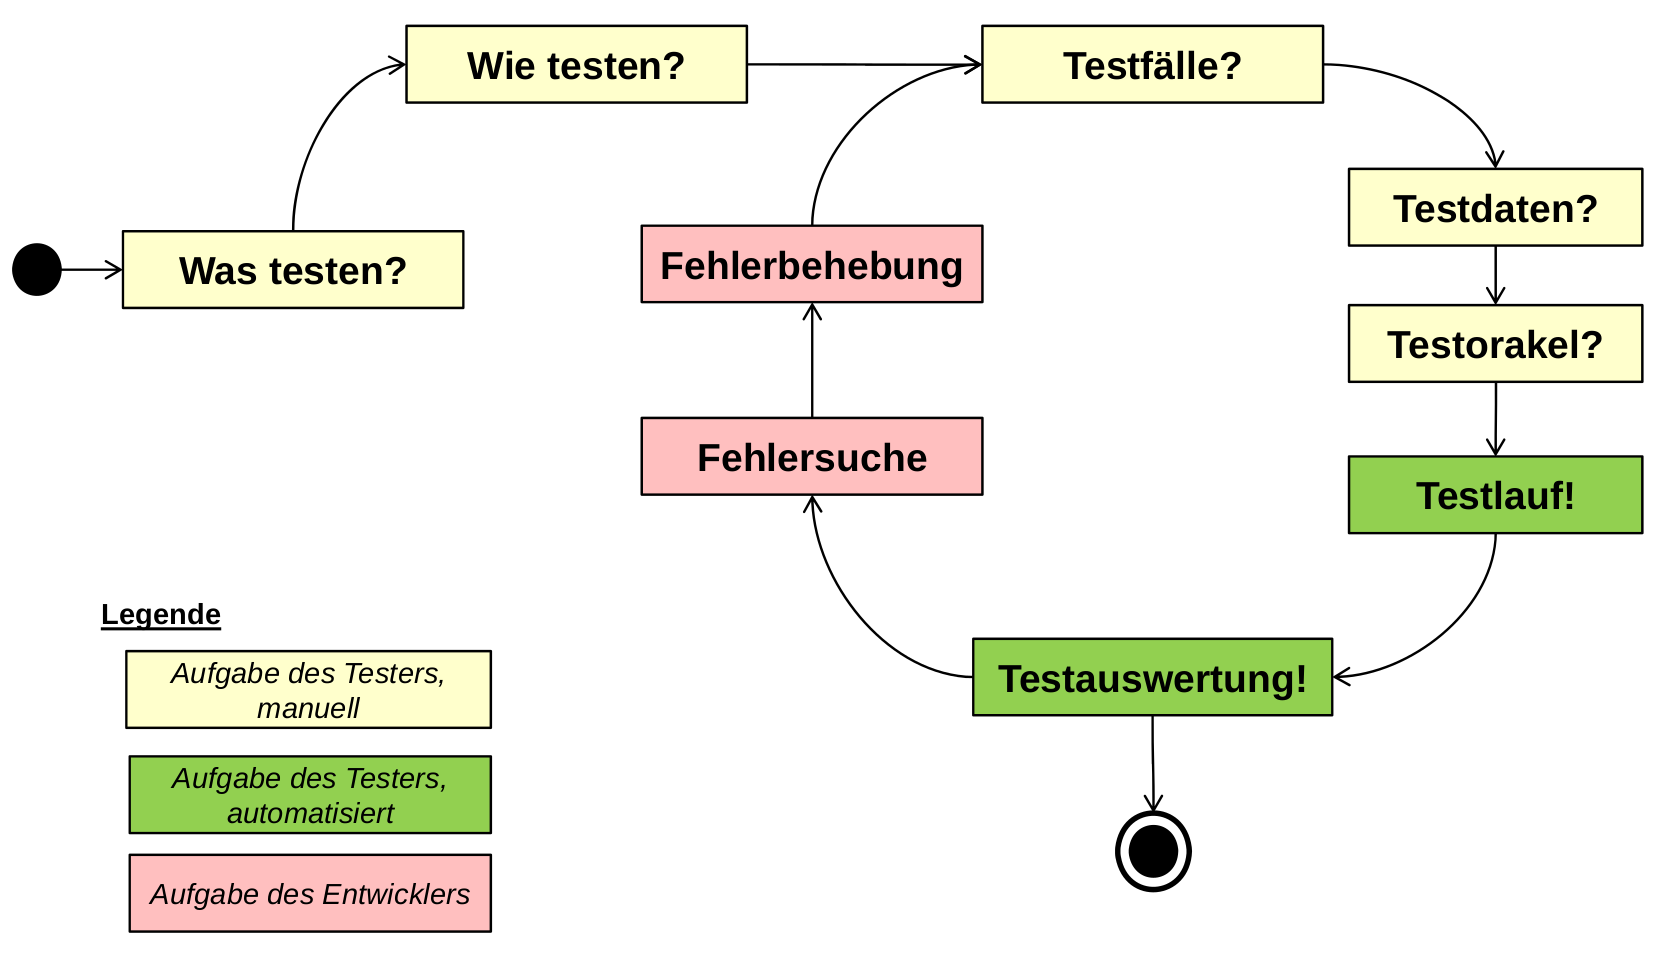
\includegraphics[width=\textwidth]{testlebenszyklus}
    \end{center}
  \end{figure}
\end{frame}


\begin{frame}
  \frametitle{Lebenszyklus Tests}
  \framesubtitle{1. Was testen?}

  \begin{figure}
    \begin{center}
      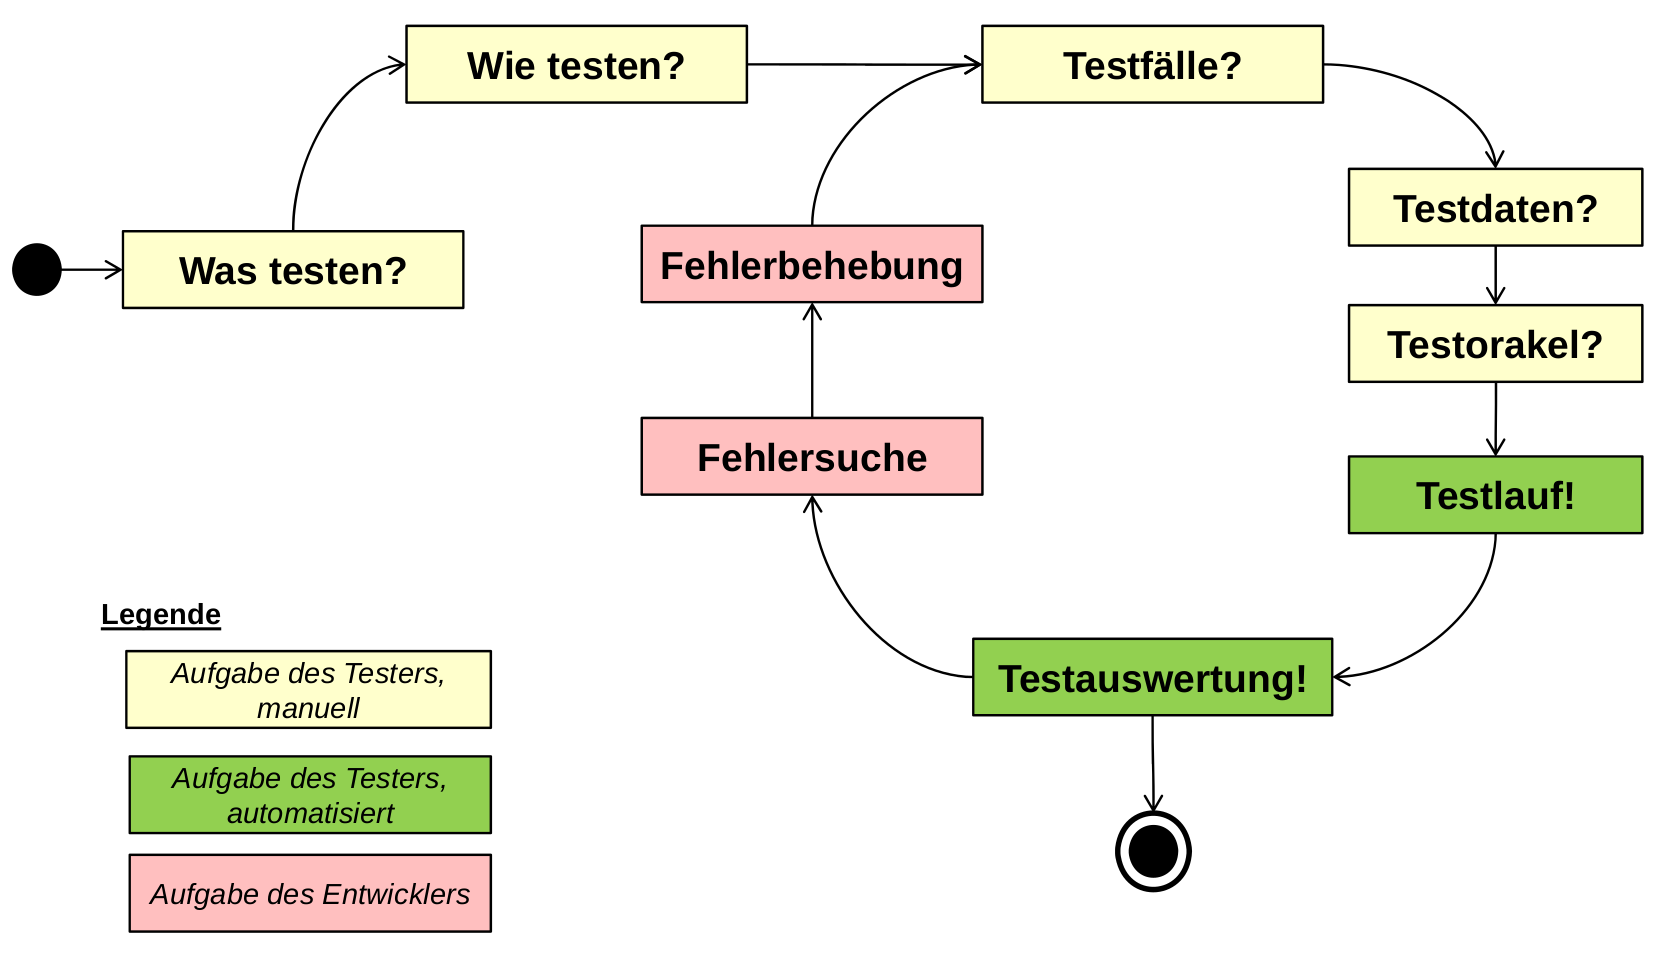
\includegraphics[height=0.5\textheight]{testlebenszyklus}
    \end{center}
  \end{figure}
  Testgegenstand: Bestimme was getestet werden soll
  \begin{itemize}
    \item Vollständigkeit der Anforderungen, \dots
    \item Testen des Codes auf Zuverlässigkeit, \dots
  \end{itemize}
\end{frame}


\begin{frame}
  \frametitle{Lebenszyklus Tests}
  \framesubtitle{2. Wie testen?}

  \begin{figure}
      \begin{center}
      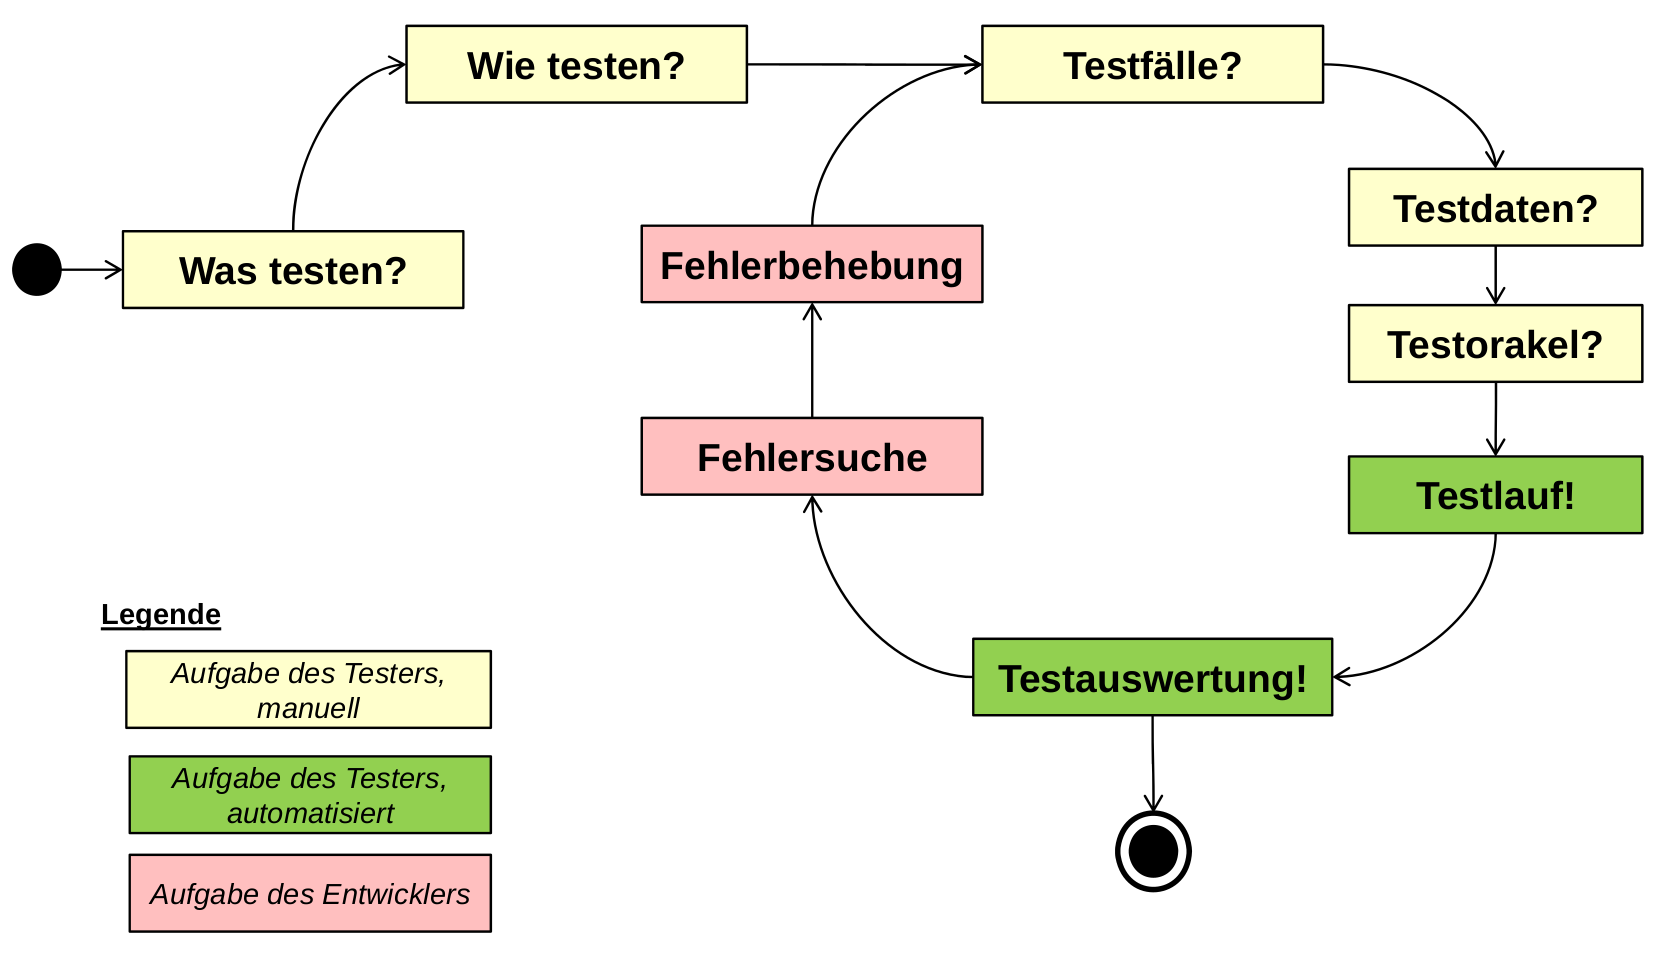
\includegraphics[height=0.5\textheight]{testlebenszyklus}
    \end{center}
  \end{figure}
  Testverfahren: Entscheide wie getestet wird
  \begin{itemize}
    \item Inspektion des Codes, \dots, Beweise
    \item Black-box, White-box
    \item Strategie für Integrationstests
  \end{itemize}
\end{frame}


\begin{frame}
  \frametitle{Lebenszyklus Tests}
  \framesubtitle{3. Testfälle}

  \begin{figure}
    \begin{center}
      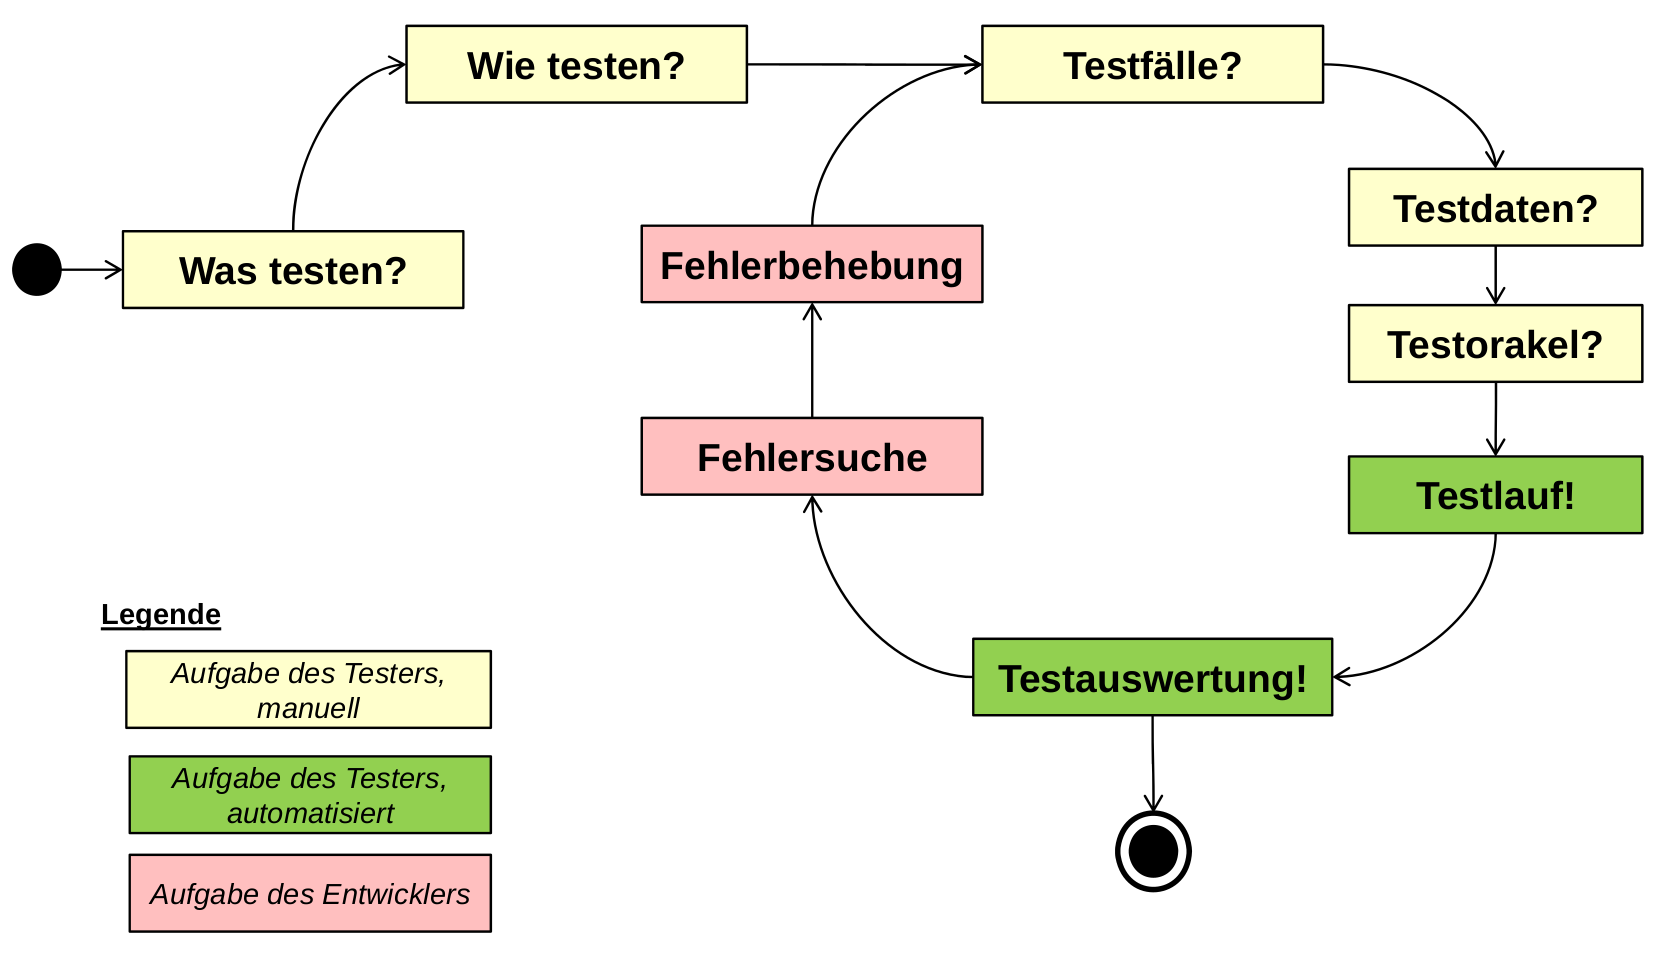
\includegraphics[height=0.5\textheight]{testlebenszyklus}
    \end{center}
  \end{figure}
  Testfälle: Entscheide was genau getestet wird
  \begin{itemize}
    \item Ein Testfall ist eine Menge von Testdaten oder Situationen, die benutzt
    werden um die zu testende Einheit (Code, Modul, System) oder das
    gemessene Attribut zu überprüfen
  \end{itemize}
\end{frame}


\begin{frame}
  \frametitle{Lebenszyklus Tests}
  \framesubtitle{4. Testdaten}

  \begin{figure}
    \begin{center}
      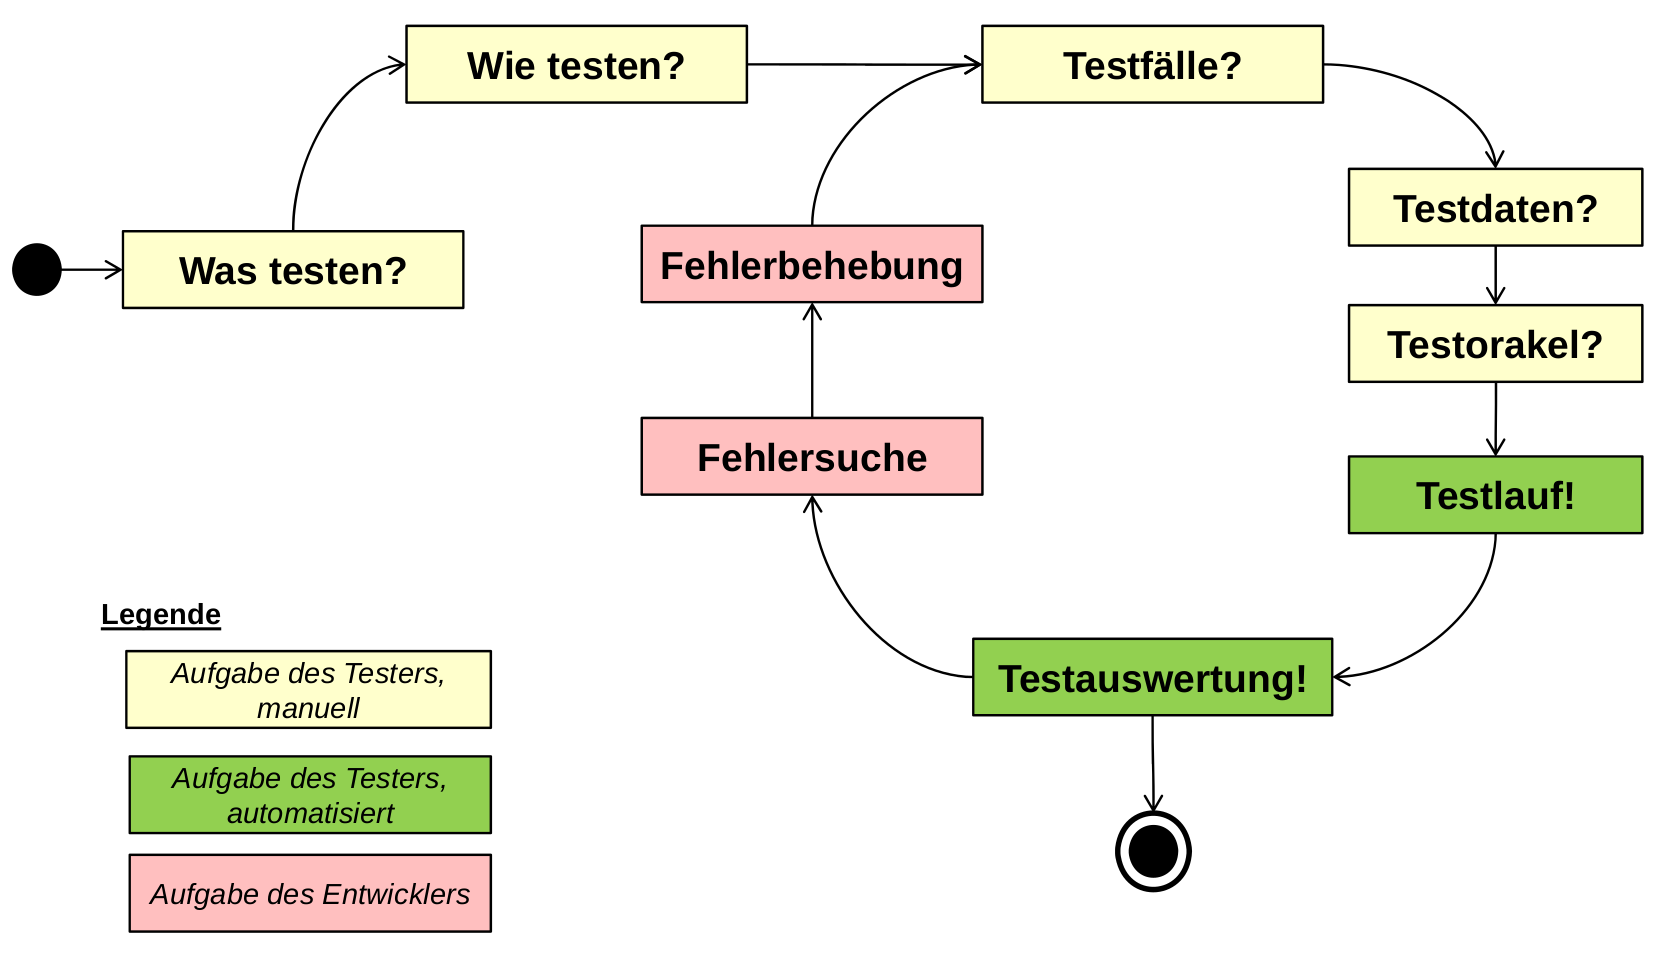
\includegraphics[height=0.5\textheight]{testlebenszyklus}
    \end{center}
  \end{figure}
  Testdaten: Entscheide wie der Testfall charakterisiert werden kann
  \begin{itemize}
    \item Daten, die einem bestimmten Testfall entsprechen
  \end{itemize}
\end{frame}


\begin{frame}
  \frametitle{Lebenszyklus Tests}
  \framesubtitle{5. Testorakel}

  \begin{figure}
    \begin{center}
      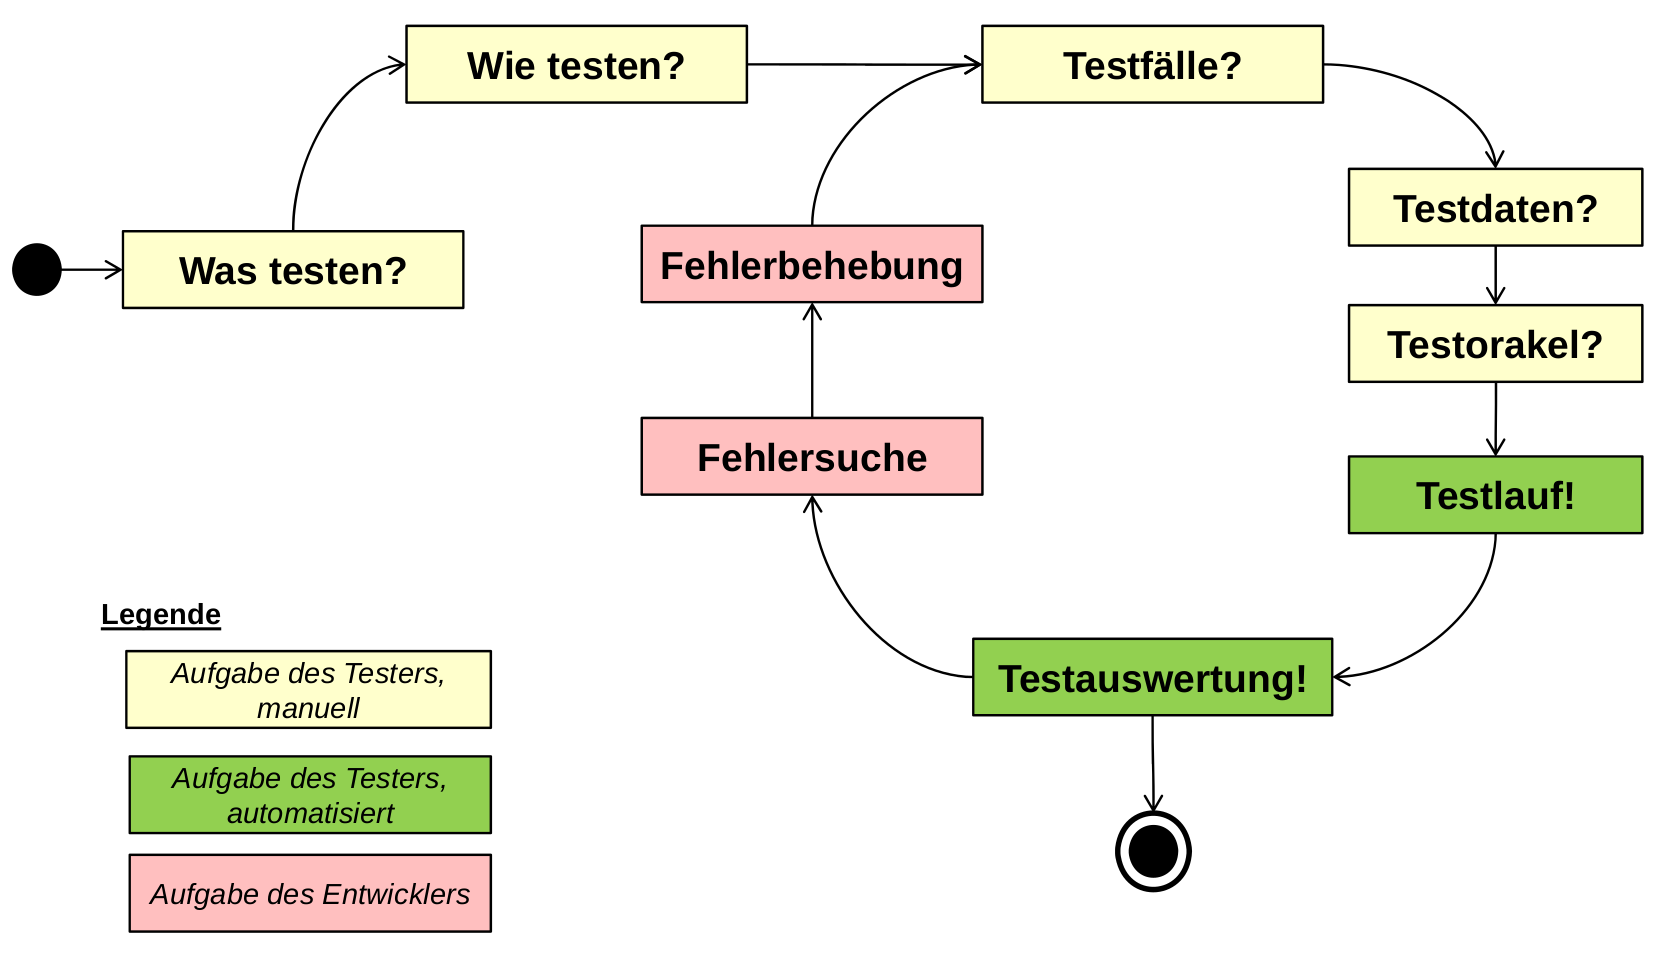
\includegraphics[height=0.5\textheight]{testlebenszyklus}
    \end{center}
  \end{figure}
  Testorakel: Entscheide anhand wovon der Testerfolg geprüft wird
  \begin{itemize}
    \item Ein Orakel besteht aus den vorhergesagten Ergebnissen für eine Menge
    von Testfällen
    \item Das Testorakel muss geschrieben werden, bevor das eigentliche Testen
    stattfindet
  \end{itemize}
\end{frame}


\begin{frame}
  \frametitle{Lebenszyklus Tests}
  \framesubtitle{6. Testlauf}

  \begin{figure}
    \begin{center}
      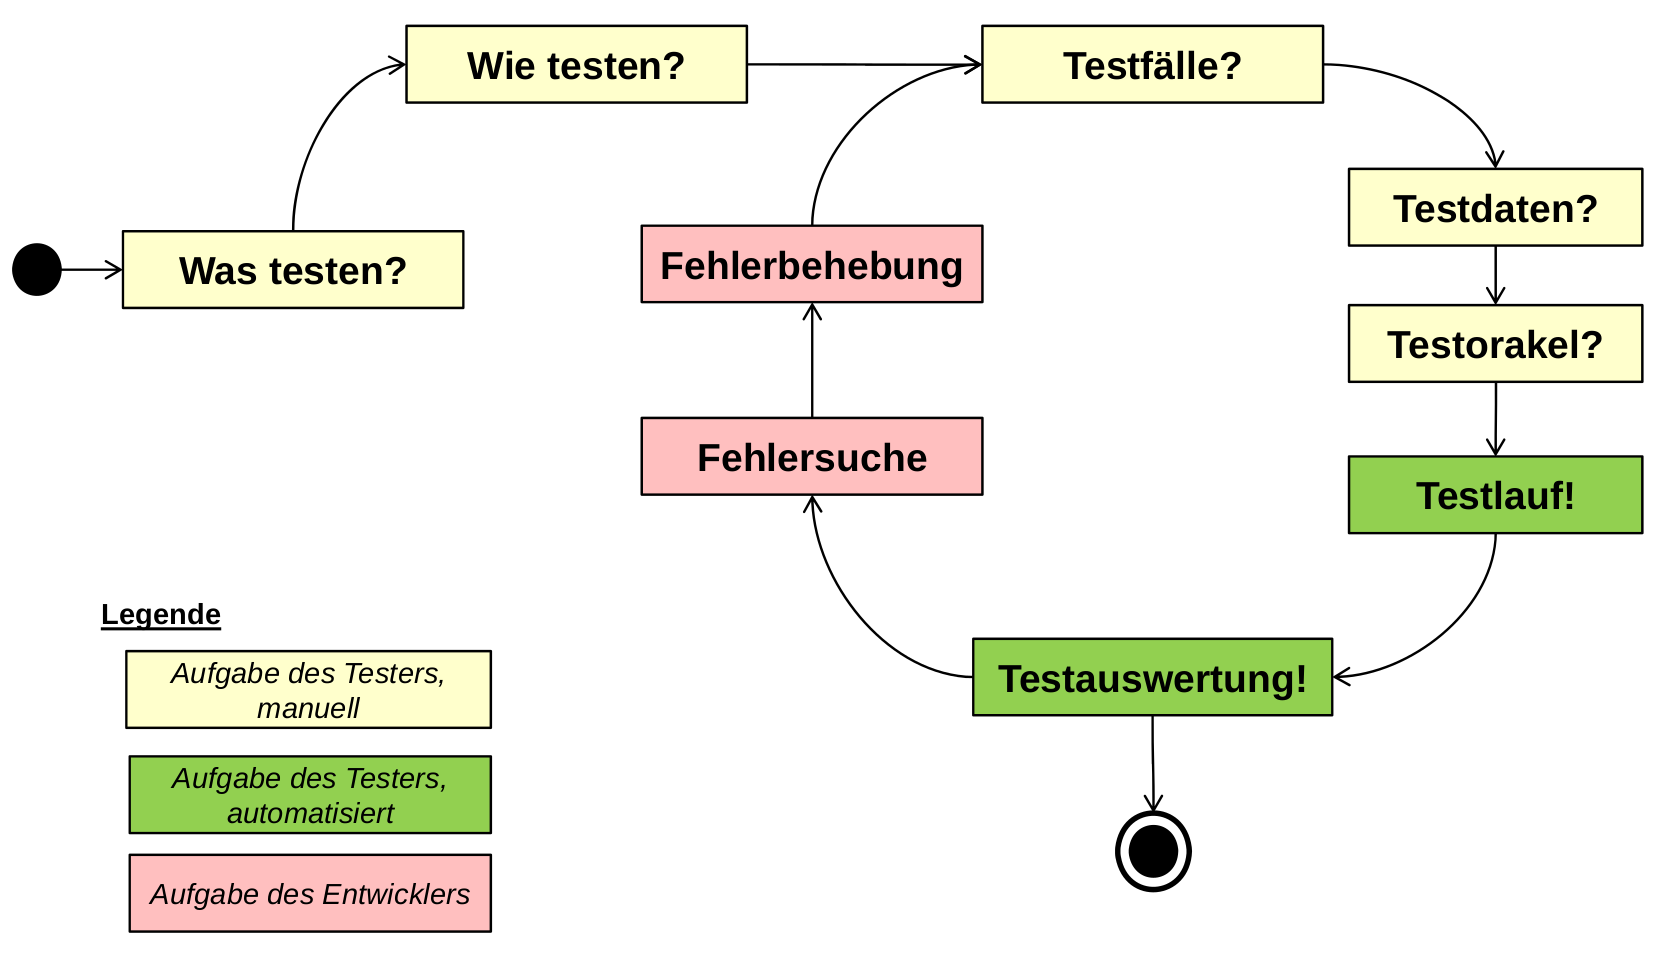
\includegraphics[height=0.5\textheight]{testlebenszyklus}
    \end{center}
  \end{figure}
  Testlauf
  \begin{itemize}
    \item Die eigentliche Ausführung des Tests und das Sammeln der
    Testergebnisse
  \end{itemize}
\end{frame}


\begin{frame}
  \frametitle{Lebenszyklus Tests}
  \framesubtitle{7. Testauswertung}

  \begin{figure}
    \begin{center}
      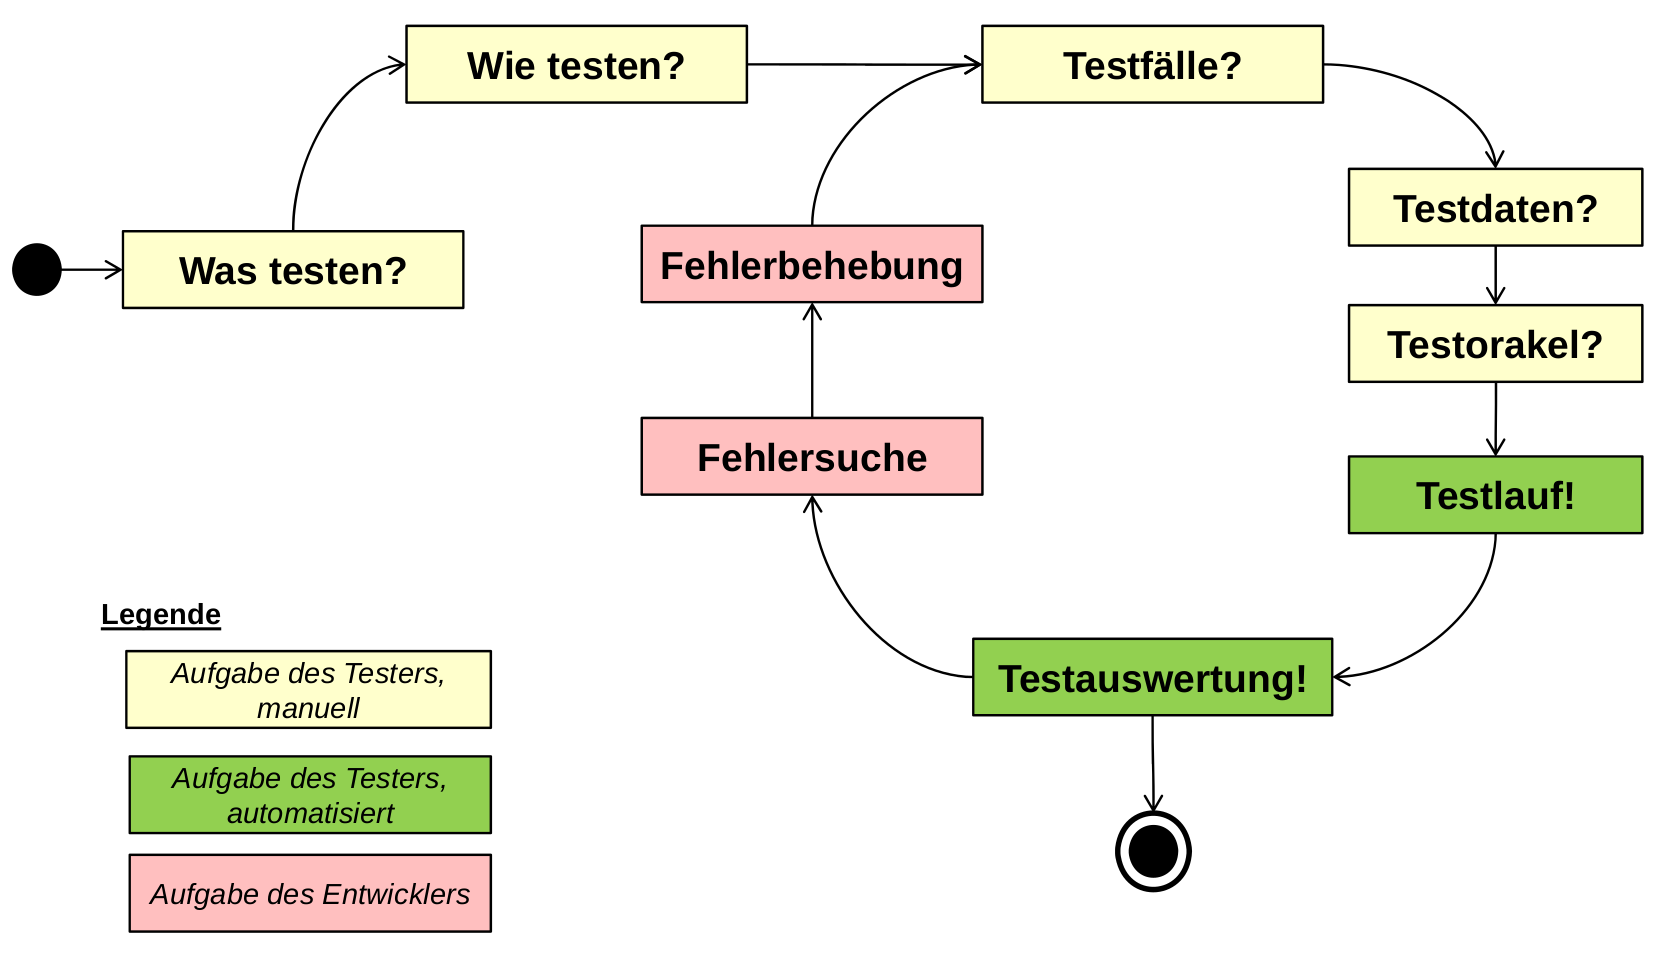
\includegraphics[height=0.5\textheight]{testlebenszyklus}
    \end{center}
  \end{figure}
  Testauswertung
  \begin{itemize}
    \item Vergleich der Testergebnisse mit dem Orakel
  \end{itemize}
\end{frame}


\begin{frame}
  \frametitle{Lebenszyklus Tests}
  \framesubtitle{Test Driven Development}

  \begin{columns}[onlytextwidth]
    \begin{column}{0.5\textwidth}
      \begin{figure}
          \begin{center}
            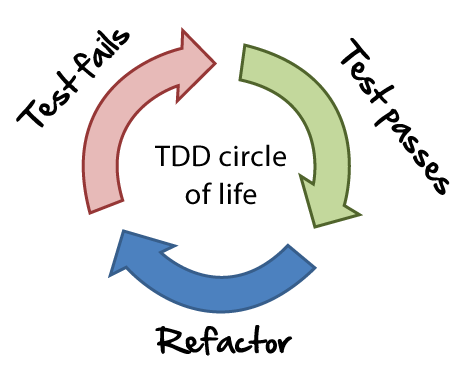
\includegraphics[height=0.5\textheight]{tdd-circle-of-life}
          \end{center}
        \end{figure}
    \end{column}
    \begin{column}{0.5\textwidth}
      \begin{itemize}
        \item<1-> Schreibe einen neuen Tests\dots
        \begin{itemize}
          \item<1-> der zur Spezifikation passt
          \item<1-> rot wird
        \end{itemize}
        \item<2-> Fix den Code im Sinne der Spezifikation bis alle Tests Grün werden
        \item<3-> Passe die Tests an
        \begin{itemize}
          \item<3-> Äquivalenzklassen zusammenfassen
          \item<3-> Gemeinsam genutzte Logik extrahieren
        \end{itemize}
      \end{itemize}
    \end{column}
  \end{columns}
\end{frame}


\begin{frame}[label=fragen]
  \frametitle{Fragen}
  \framesubtitle{Fragen?}
  \begin{figure}
    \begin{center}
      
\includegraphics[height=4cm]{fragen}
    \end{center}
  \end{figure}
\end{frame}


\section{Unit Tests}
\subsection{Begriffsklärung}


\begin{frame}
  \frametitle{Begriffsklärung}
  \framesubtitle{Definition Unit Test}

  \begin{definition}[Unit Test]
  Ein \highlighton{Unit Test} (auch Modultest oder Komponententest) wird in der Softwareentwicklung angewendet, um die funktionalen \highlighton{Einzelteile} (Module) von Computerprogrammen zu testen, d. h., sie auf korrekte Funktionalität zu prüfen.
  \end{definition}
\end{frame}


\begin{frame}
  \frametitle{Begriffsklärung}
  \framesubtitle{Eigenschaften Unit Tests}
  \begin{itemize}
    \item<1-> Konsistent
    \item<2-> Eindeutig
    \item<3-> Testet ein Subjekt
    \item<4-> Testet einen Testfall
    \item<5-> Ohne eigene Logik oder Schleifen
    \item<6-> Präzise Annahmen
    \item<7-> Selbsterklärend
  \end{itemize}
\end{frame}


\begin{frame}
  \frametitle{Begriffsklärung}
  \framesubtitle{Wirkung der Eigenschaften}

  \begin{itemize}
    \item<1-> Begrenzt komplex durch Fokus auf Modul
    \item<2-> Klar definierte Schnittstellen
    \item<3-> Senkt die Komplexität von Integrationstests
    \begin{itemize}
      \item<3-> Integrationstest können stichprobenartig durchgeführt werden
    \end{itemize}
    \item<4-> Es stehen verschiedene Strategien zur Ermittlung von Testfällen zur Verfügung
  \end{itemize}
\end{frame}


\againframe{fragen}


\subsection{Testfallauswahl}
\subsubsection{Black-box Tests}


\begin{frame}
  \frametitle{Black-box Tests}
  \framesubtitle{Eigenschaften Black-box Tests}
  \begin{itemize}
    \item<1-> Testfallauswahl anhand von Analysewissen über funkt. Anforderungen
    \begin{itemize}
      \item<2-> Use cases
      \item<3-> Erwartete Eingabedaten
      \item<4-> Ungültige Eingabedaten
    \end{itemize}
    \item<5-> Fokus: Ein-/Ausgabeverhalten
    \begin{itemize}
      \item<6-> Das Modul besteht den Test, wenn für jede gegebenen Eingabe die
      Ausgabe vorhersagbar ist
      \item<7-> Es ist meist unmöglich, jede mögliche Eingabe zu erzeugen („test cases“)
    \end{itemize}
  \end{itemize}
\end{frame}


\begin{frame}
  \frametitle{Black-box Tests}
  \framesubtitle{Partitionierung}
  \begin{itemize}
    \item<1-> Reduzierung der Anzahl der Testfälle durch Partitionierung
    \begin{itemize}
      \item<2-> Zerlege Eingabe in Äquivalenzklassen
      \item<3-> Wähle Testfälle für jede der Äquivalenzklassen.
      (Beispiel: Wenn ein Objekt negativen Zahlen akzeptieren soll, reicht es
      aus, mit einer negativen Zahl zu testen)
    \end{itemize}
  \end{itemize}
\end{frame}


\begin{frame}
  \frametitle{Black-box Tests}
  \framesubtitle{Partitionierung}

  Wahl der Partitionierung (Richtlinie)
  \begin{itemize}
    \item<1-> Gültige Eingabewerte liegen in einem Intervall. Wähle Testfälle aus drei Äquivalenzklassen
    \begin{itemize}
      \item<1-> Unterhalb des Intervalls
      \item<2-> Im Intervall
      \item<3-> Oberhalb des Intervalls
    \end{itemize}
    \item<4-> Gültige Eingabewerte bilden eine diskrete Menge. Wähle Testfälle aus
    zwei Äquivalenzklassen:
    \begin{itemize}
      \item<5-> Gültiger diskreter Wert
      \item<6-> Ungültiger diskreter Wert
    \end{itemize}
  \end{itemize}

\end{frame}


\begin{frame}[fragile]
  \frametitle{Black-box Tests}
  \framesubtitle{Beispiel}
  \begin{block}{Contract}
    Verbindet die beiden Werte mit Hilfe des Operators und gibt das Ergebnis zurück.
  \end{block}

  \begin{minted}[firstline=2,linenos=false]{php}
    <?php
    class Calculator
    {
      /**
      * @param float $a
      * @param float $b
      * @param Operator $operator
      *
      * @return mixed
      */
      public function calculateBinaryOperation($a, $b, Operator $operator)
    }
  \end{minted}
\end{frame}


\begin{frame}[fragile]
  \frametitle{Black-box Tests}
  \framesubtitle{Beispiel}
  \begin{block}{Contract}
    Diese Klasse implementiert die Division.
  \end{block}

  \begin{minted}[firstline=2,linenos=false]{php}
    <?php
    class Calculator
    {
      /**
      * @param float $a
      * @param float $b
      *
      * @return float
      */
      public function division($a, $b)
    }
  \end{minted}
\end{frame}


\againframe{fragen}


\subsubsection{White-box Tests}


\begin{frame}
  \frametitle{White-box Tests}
  \framesubtitle{Definition White-box Tests}

  \begin{definition}[White-box Tests]
    Der Begriff \highlighton{White-Box-Test} (seltener auch Glass-Box-Test) bezeichnet eine Methode des Software-Tests, bei der die Tests mit Kenntnissen über die \highlighton{innere Funktionsweise} des zu testenden Systems entwickelt werden.
  \end{definition}
\end{frame}


\begin{frame}
  \frametitle{White-box Tests}
  \framesubtitle{Ziel von White-box Tests}

  Wissen über Entwurf und Implementierung nutzen um \dots
  \begin{itemize}
    \item<1-> Anzahl von Testfällen zu begrenzen
    \item<2-> Gründliche Testabdeckung zu gewährleisten
  \end{itemize}
\end{frame}


\begin{frame}
  \frametitle{White-box Tests}
  \framesubtitle{Ziel von White-box Tests}
  Testfallauswahl
  \begin{itemize}
    \item<1-> Entwurfswissen über Systemaufbau, Algorithmen, Datenstrukturen
    \item<2-> Kontrollstrukturen: Verzweigungen, Schleifen, \dots
    \item<3-> Datenstrukturen: Datensätze, Felder, Arrays, \dots
  \end{itemize}
\end{frame}




\begin{frame}
  \frametitle{White-box Tests}
  \framesubtitle{Abdeckung}
  \begin{definition}[Testabdeckung]
    Abdeckung ist prozentuales Maß der vom Test durchlaufenen Teile der
    getesteten Komponente im \highlighton{Verhältnis zur Gesamtanzahl} solcher Teile.
    \begin{equation*}
    Abdeckung = \dfrac{Anzahl getesteter Teile}{Anzahl aller Teile}
    \end{equation*}
  \end{definition}
  \pause
  Zu testende Teile
  \begin{itemize}
    \item<2-> jede Anweisung \(rightarrow\) Anweisungsabdeckung
    \item<3-> jede Verzweigung \(rightarrow\) Verzweigungsabdeckung
    \item<4-> jede Schleife \(rightarrow\) Schleifenabdeckung
    \item<5-> jeder Pfad \(rightarrow\) Pfadabdeckung
  \end{itemize}
\pause[6]
Ein „Teil“ gilt als getestet wenn es während des Testlaufs mindestens
einmal durchlaufen wurde
\end{frame}


\begin{frame}[fragile]
  \frametitle{White-box Tests}
  \framesubtitle{Anweisungsabdeckung}

  Nicht einfach, 100\% Anweisungsabdeckung zu erreichen
  \begin{itemize}
    \item<1-> Fehlerbedingungen / seltene Ereignisse:
      \begin{lstlisting}
    if (param > 20) {
      print("Dies sollte nie geschehen!");
    }
      \end{lstlisting}
    \item<2-> Exceptions inmitten einer Anweisungsfolge:
      \begin{lstlisting}
  doThis(); # throws exception
  doThat(); # never reached
      \end{lstlisting}
  \end{itemize}

  \pause[3]

  \begin{center}
    Eine Anweisung ist abgedeckt, wenn sie ausgeführt wird.\\
    Anweisung != Codezeile
  \end{center}

\end{frame}


\begin{frame}[fragile]
\frametitle{White-box Tests}
\framesubtitle{Verzweigungsabdeckung}

\begin{itemize}
  \item Prüft alle Alternativen einer Verzweigung
  \item Schützt vor Fehlern, die dadurch entstehen, dass bestimmte Anforderungen in einem Zweig nicht erfüllt sind.
\end{itemize}


  \begin{columns}[onlytextwidth]
      \begin{column}{0.5\textwidth}
      \begin{lstlisting}
$divisor = 0;

if ($flag){$divisor = 1;}
else {     $divisor = 0;}

echo 3 / $divisor;
      \end{lstlisting}
    \end{column}
    \begin{column}{0.5\textwidth}
        Der Code wirft eine Exception, falls \lstinline|$flag| gleich false ist.
    \end{column}
  \end{columns}
\end{frame}


\begin{frame}[fragile]
\frametitle{White-box Tests}
\framesubtitle{Verzweigungsabdeckung}

Fehlendes else ist auch ein Zweig der getestet werden muss!

\begin{lstlisting}
$divisor = 0;
if ($flag){$divisor = 1;}
echo 3 / $divisor;
\end{lstlisting}

\begin{block}{Fun Fact}<2->
  100\% Verzweigungsabdeckung impliziert 100\% Anweisungsabdeckung, sofern das Programm \highlighton{keine Exception}wirft.
\end{block}

\end{frame}


\begin{frame}[fragile]
\frametitle{White-box Tests}
\framesubtitle{Grenzen der Verzweigungsabdeckung}

Es gibt Fehlerklassen, die durch Verzweigungsabdeckung nicht
erkannt werden.

\begin{lstlisting}<1->
$value = null;
if ($a) { $value = new DateTime(); }
if ($b) { $value->format('Y');}
\end{lstlisting}

\begin{itemize}
  \item<2-> 100\% Verzweigungsabdeckung ist gegeben, wenn (\$a, \$b) mit
  (true, true) und (false, false) belegt wird
  \item<3-> Für (\$a, \$b) = (false, true) gibt‘s einen Zugriff auf null \(\rightarrow\) Exception
\end{itemize}
\end{frame}


\begin{frame}[fragile]
\frametitle{White-box Tests}
\framesubtitle{Pfadabdeckung}

\begin{description}
  \item<1->[Ziel] der Pfadabdeckung ist das Durchlaufen des Programmes auf jedem mögliche Pfad.
  \begin{lstlisting}<2->
  $value = null;
  if ($a) { $value = new DateTime(); }
  if ($b) { $value->format('Y');}
  \end{lstlisting}
  \begin{itemize}
    \item<2-> Verfügbare Pfade \lstinline|(\$a, \$b) = (true,true),(false,true),(true,false),(false,false)|
  \end{itemize}
  \item<3->[Pfad] ist jeder Weg von Startpunkt zum Endpunkt im
  Kontrollflussgraphen des analysierten Codes
  \begin{itemize}
    \item<4-> Return-Anweisungen haben Kanten zum Endpunkt
    \item<5-> Exceptions nicht \(\rightarrow\) sie stellen kein "normales“ Ende dar!
    \item<6-> Fehlende else-Anweisungen zählen als Kanten im Graphen
    \begin{itemize}
      \item<7-> In obigem Beispiel ist gerade der "fehlende“ Zweig a=false kritisch!
    \end{itemize}
  \end{itemize}
\end{description}
\end{frame}

\begin{frame}
  \frametitle{White-box Tests}
  \framesubtitle{Grenzen der Pfadabdeckung}

  \begin{block}{Halteproblem}
    \begin{description}
      \item[Problem:] Zyklen können zu einer unendlichen Anzahl von Pfaden führen.
      \item[Lösung:] Pfade durch ein und den selbe Zyklus kollabieren zu einer Äquivalenzklasse.
    \end{description}
  \end{block}
  \pause
  \begin{block}{Zu viele Pfade}
    \begin{description}
      \item[Problem:] Der Programmcode ist zu komplex.
      \item[Folgerung:] Anderes Testverfahren wählen oder Komplexität reduzieren.
    \end{description}
  \end{block}
\end{frame}


\begin{frame}
\frametitle{White-box Tests}
\framesubtitle{Verzweigungsabdeckung}

\begin{block}{Fun Fact}
  \begin{center}
    100\% \highlighton{Pfadabdeckung} \\
    impliziert \\
    100\% \highlighton{Verzweigungsabdeckung} \\
    und \\
    100\% \highlighton{Anweisungsabdeckung}
  \end{center}
\end{block}
\end{frame}


\begin{frame}[fragile]
  \frametitle{White-box Tests}
  \framesubtitle{Verzweigungsabdeckung}

  \begin{minted}{java}
    FindMean (FILE ScoreFile) {
      int NumberOfScores = 0; //1
      float SumOfScores = 0.0; //1
      float Mean = 0.0; //1
      float Score; //1
      Read(ScoreFile, Score); //1
      while ( !EOF(ScoreFile) ) { //2
        if (Score > 0.0 ) { //3
          SumOfScores = SumOfScores + Score; //4
          NumberOfScores++; //4
        } //5
        Read(ScoreFile, Score); //6
      }
      /* Compute the mean and print the result */
      if (NumberOfScores > 0) { //7
        Mean = SumOfScores / NumberOfScores; //8
        printf(" The mean score is %f\n", Mean); //8
      } else printf ("No scores found in file\n"); //9
    }
  \end{minted}
\end{frame}


\begin{frame}[fragile]
\frametitle{White-box Tests}
\framesubtitle{Verzweigungsabdeckung}

\begin{figure}
      \begin{center}
        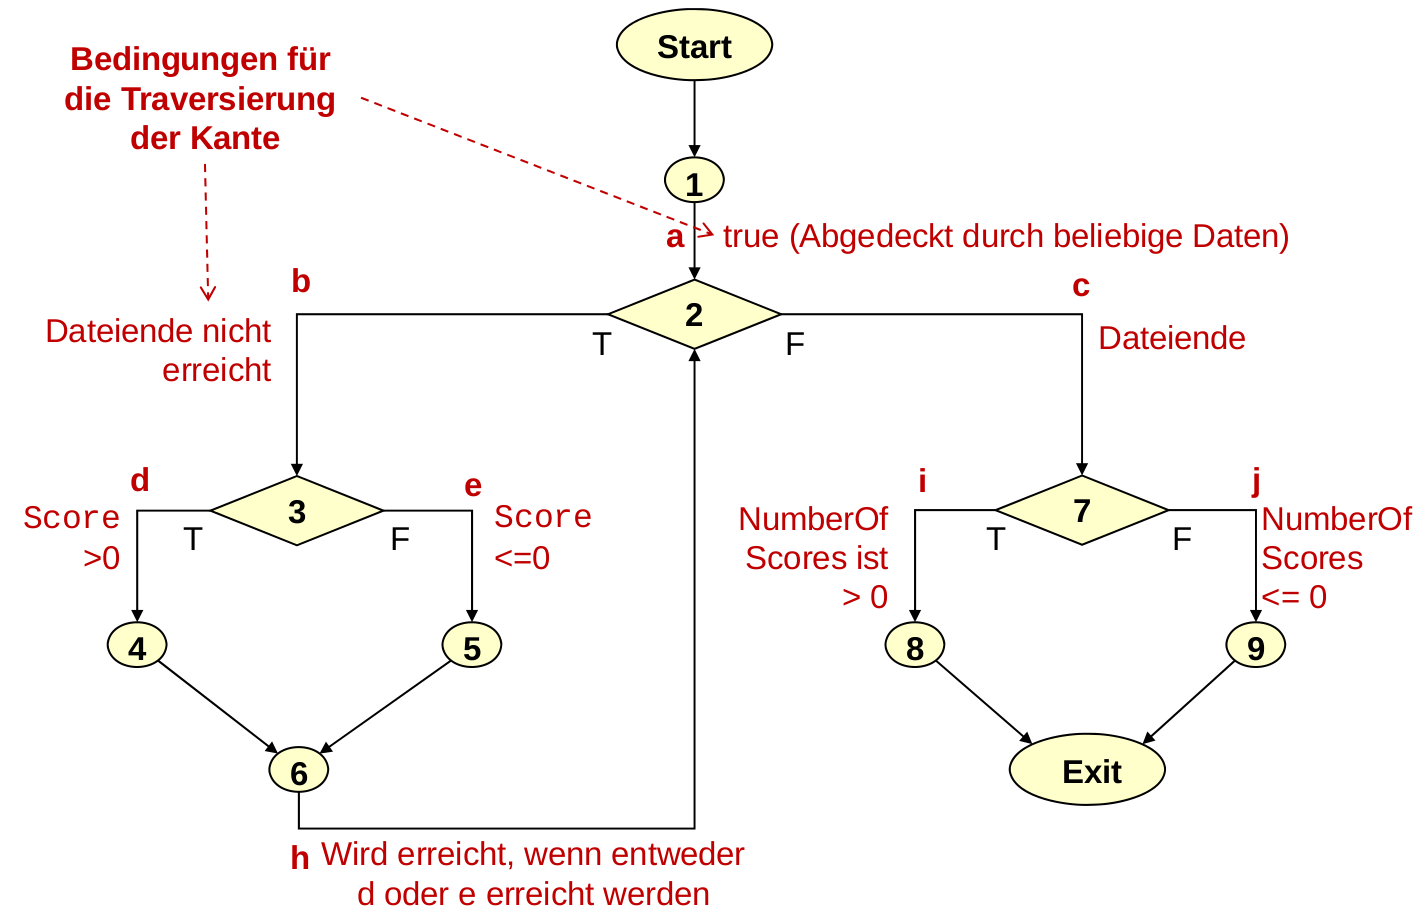
\includegraphics[width=\textwidth]{pfaddiagramm1}
      \end{center}
    \end{figure}
\end{frame}


\begin{frame}[fragile]
\frametitle{White-box Tests}
\framesubtitle{Verzweigungsabdeckung}

\begin{figure}
  \begin{center}
    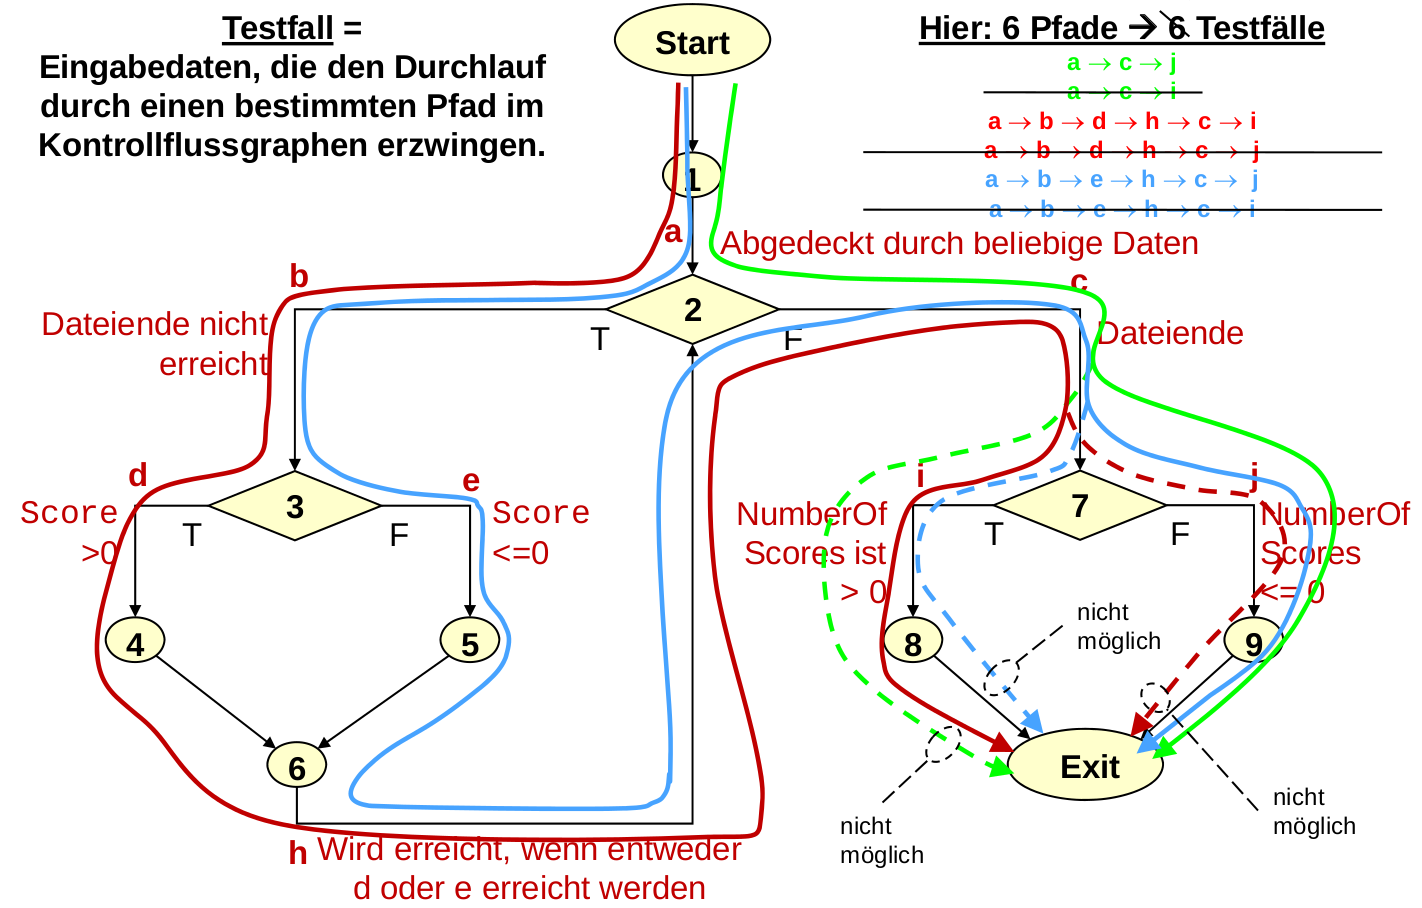
\includegraphics[width=\textwidth]{pfaddiagramm2}
  \end{center}
\end{figure}
\end{frame}


\begin{frame}[fragile]
\frametitle{White-box Tests}
\framesubtitle{Verzweigungsabdeckung}

\begin{figure}
  \begin{center}
    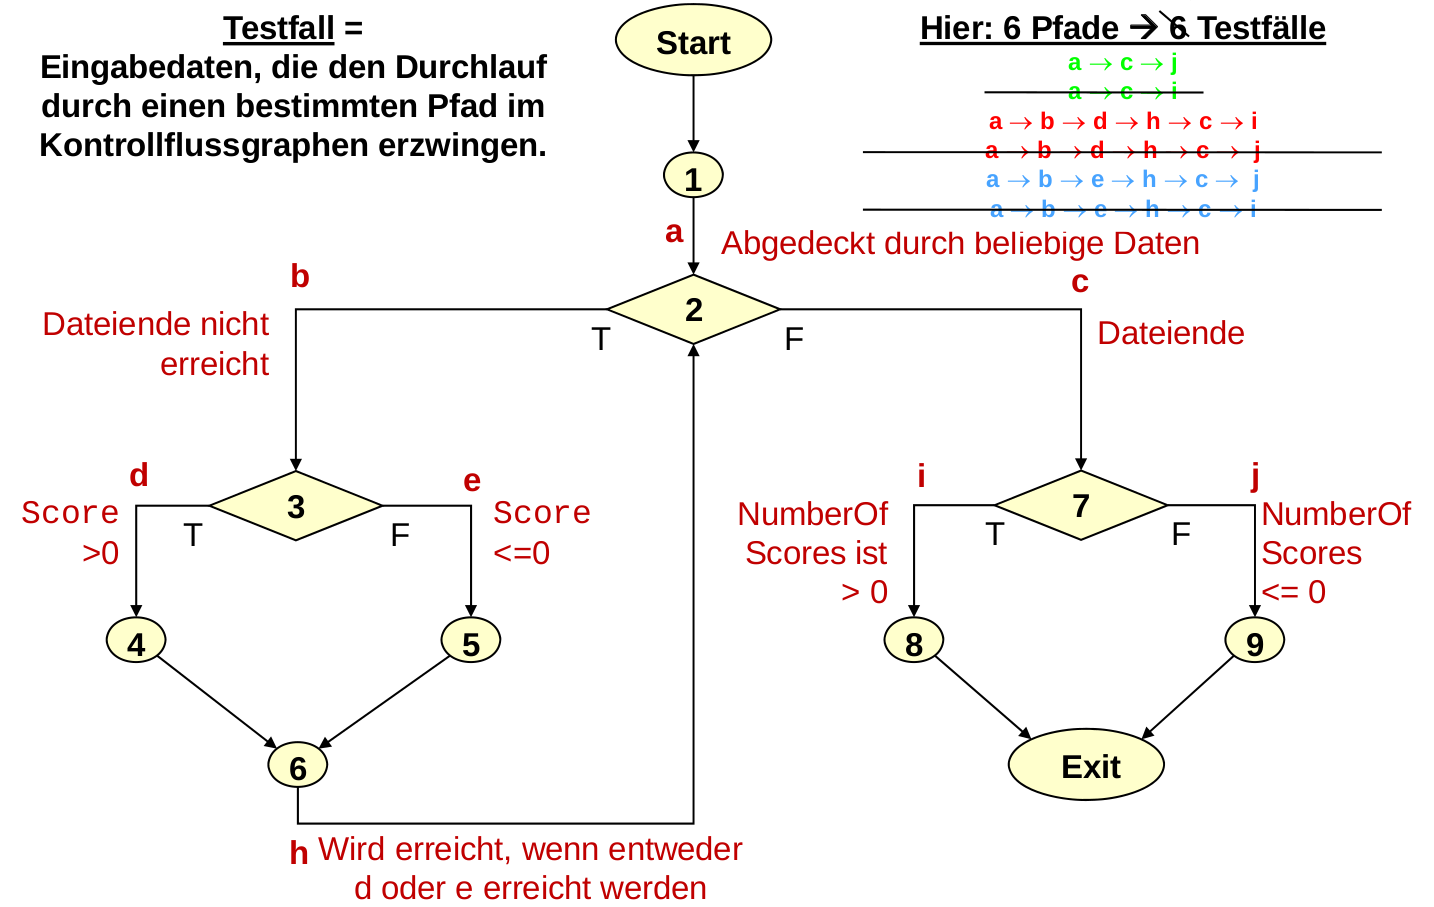
\includegraphics[width=\textwidth]{pfaddiagramm3}
  \end{center}
\end{figure}
\end{frame}


\begin{frame}[fragile]
\frametitle{White-box Tests}
\framesubtitle{Verzweigungsabdeckung}

\begin{figure}
  \begin{center}
    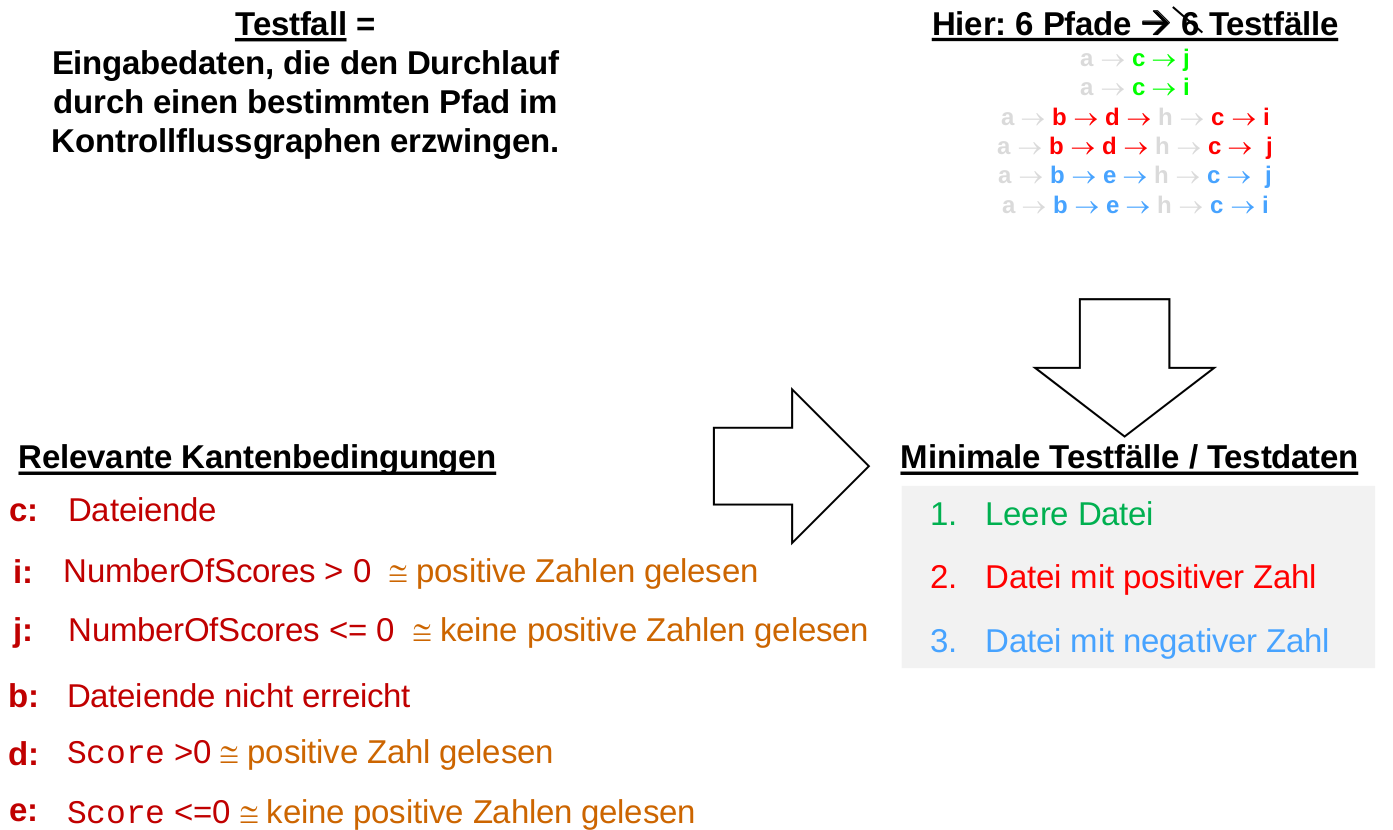
\includegraphics[width=\textwidth]{pfadtestfaelle}
  \end{center}
\end{figure}
\end{frame}


\begin{frame}[fragile]
\frametitle{White-box Tests}
\framesubtitle{Verzweigungsabdeckung}

\begin{enumerate}
  \item Kontrollflussgraphen erstellen
  \item Kanten beschriften
  \item Pfade bestimmen
  \item Unmögliche Pfade eliminieren
  \item Kanten die keine Bedingung mit sich tragen eliminieren
  \item Kanten, deren Bedingung durch die vorangegangenen Schritte erfüllt wurden eliminieren
  \item Eingabedaten bestimmen, die die Bedingungen der restlichen Kanten  erfüllen
  \item Testdatensatz erzeugen
  \item Testorakel dafür erzeugen
  \item Kontrollflussgraphen erstellen
\end{enumerate}
\end{frame}

\begin{frame}[fragile]
  \frametitle{White-box Tests}
  \framesubtitle{Übung}

  \begin{minted}[firstline=2]{php}
    <?php
    public function findIntersection(&$firstSet, &$secondSet) {
      if (!is_array($firstSet) || !is_array($secondSet)) { #1
        return $firstSet === $secondSet; #2
      } #3

      $commonKeys  = array_intersect(array_keys($firstSet), array_keys($secondSet)); #4
      $returnValue = array(); #5
      foreach ($commonKeys as $key) { #6
        $intersection = $this->findIntersection($firstSet[$key], $secondSet[$key]); #7
        if ($intersection !== array()) { #8
          $returnValue[$key] = $intersection; #9
        } #10
      } #11
      return $returnValue; #12
    }
  \end{minted}
\end{frame}


\begin{frame}[fragile]
\frametitle{White-box Tests}
\framesubtitle{Verzweigungsabdeckung}

\begin{figure}
  \begin{center}
    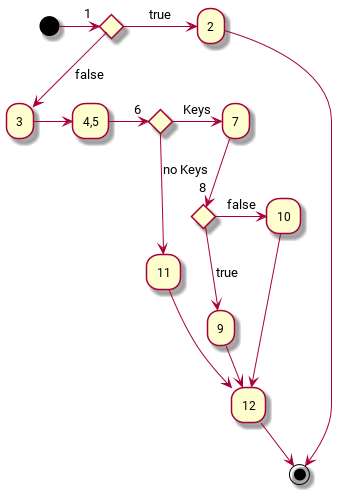
\includegraphics[height=7cm]{activity_alt}
  \end{center}
\end{figure}
\end{frame}


\againframe{fragen}


\begin{frame}[fragile]
\frametitle{White-box vs Black-box}
\framesubtitle{Zusammenfassung}

\begin{columns}[onlytextwidth]
  \begin{column}{0.5\textwidth}
    \begin{block}<1->{White-box}
      \begin{itemize}
        \item Potentiell unendliche Anzahl von Pfaden muss getestet werden
        \item Getestet wird anhand der tatsächlich anstatt des erwarteten Verhaltens
        \item Keine Erkennung fehlender Use Cases
      \end{itemize}
    \end{block}
  \end{column}
  \begin{column}{0.5\textwidth}
    \begin{block}<2->{Black-box}
      \begin{itemize}
        \item Potentielle kombinatorische Explosion der Testfälle (gültige \& ungültige Daten)
        \item Oft ist es unklar, ob die  gewählten Testfälle einen bestimmten Fehler entdecken
        \item Keine Entdeckung belangloser Use Cases
      \end{itemize}
    \end{block}
  \end{column}
\end{columns}
\begin{block}<3->{Fact}
  White-box-Tests und Black-box-Tests sind die beiden Extreme des  Modultest-Kontinuums. Beide Testtypen sind erforderlich.
\end{block}
\end{frame}


\againframe{fragen}


\section{Code Dojo}
\subsection{Das Dojo}



{
\usebackgroundtemplate{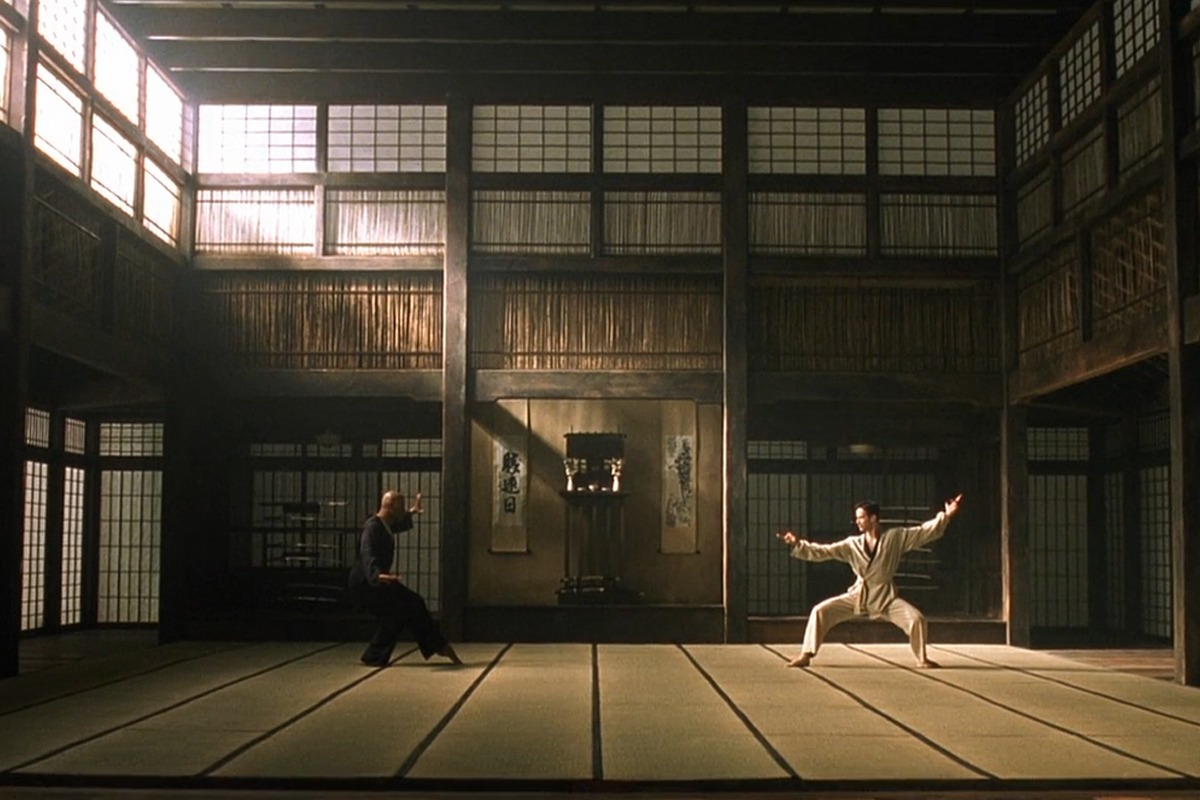
\includegraphics[height=\paperheight,width=\paperwidth]{dojo}}
\setbeamertemplate{blocks}[rounded][shadow=false]

  \begin{frame}[fragile]
    \frametitle{Code Dojo}
    \framesubtitle{Was ist ein Dojo?}
    \begin{exampleblock}{}
      Dojo (jap. Ort des Weges) bezeichnet einen Trainingsraum für verschiedene japanische Kampfkünste (Budo) [\dots]. Im übertragenen Sinne steht der Begriff auch für die Gemeinschaft der dort Übenden.
      \flushright{{\em Wikipedia}}
    \end{exampleblock}
  \end{frame}


  \begin{frame}[fragile]
    \frametitle{Code Dojo}
    \framesubtitle{Was ist ein Dojo?}

    \begin{exampleblock}{}
      Die Gemeinschaft führt gemeinsam Übungen -- so genannte Katas -- durch um ihr Wissen in der entsprechenden Disziplin zu vervollkommnen.
    \end{exampleblock}
  \end{frame}
}


\subsection{Code Kata}


\begin{frame}[fragile]
  \frametitle{Code Kata}
  \framesubtitle{Was ist ein Code Kata?}

  \begin{figure}
    \begin{center}
      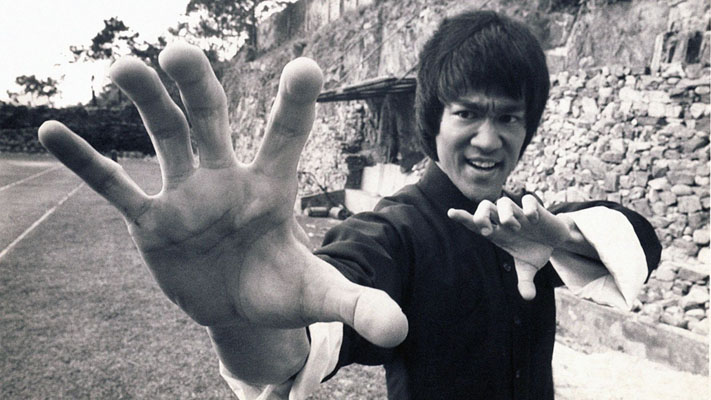
\includegraphics[width=0.7\textwidth]{bruce-lee}
    \end{center}
  \end{figure}

  \begin{itemize}
    \item<+-> Kleine, unabhängige, fokussierte, in sich geschlossene Übung
    \item<+-> Übt die Ausführung und Herangehensweise
    \item<+-> Bietet Raum für gemeinsames Lernen
    \item<+-> Lösung der Aufgabe erklärtes Nicht-Ziel
  \end{itemize}

\end{frame}


\subsection{Das Tennis Kata}

{
\usebackgroundtemplate{
\includegraphics[height=\paperheight,width=\paperwidth]{gears}}
\setbeamertemplate{blocks}[rounded][shadow=false]

\begin{frame}[fragile]
  \frametitle{Das Tennis Kata}
  \framesubtitle{Fokus}
  \begin{block}{Fokus}
    \begin{itemize}
      \item<+-> Pair Programming + TDD = TDD-Game
      \item<+-> Keine PHPMD Regel darf gebrochen werden
      \item<+-> Absichtsvolles Testen
      \begin{itemize}
        \item<+-> Test wird zuallererst dem Pair-Partner erklärt, dann programmiert
        \item<+-> Auswahl des Zwecks (use case, Erwartete Eingaben \dots)
        \item<+-> Auswahl der Kategorie (Black-, White-box)
        \item<+-> Gegebenenfalls Auswahl der Äquivalenzklasse.
      \end{itemize}
    \end{itemize}
  \end{block}

\end{frame}
}


{
\usebackgroundtemplate{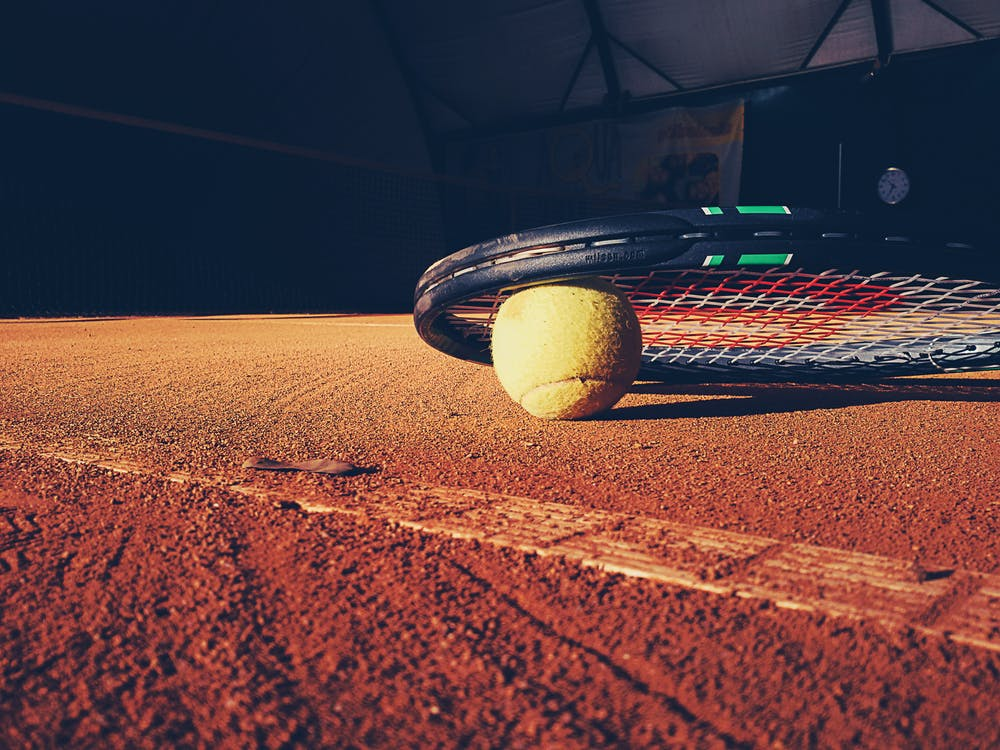
\includegraphics[width=\paperwidth]{tennis.jpg}}
\setbeamertemplate{blocks}[rounded][shadow=false]

\begin{frame}[fragile]

  \frametitle{Das Tennis Kata}
  \framesubtitle{Anforderung}

  \begin{block}{Anforderung}
    \begin{itemize}
      \item Eine Klasse muss die folgenden public Methoden haben
      \begin{itemize}
        \item \highlighton{addPointToPlayer(PlayerName:string):null} - Soll aufgerufen werden wenn ein Spieler einen Punkt erzielt. Wirft eine Exception, wenn das Spiel vorbei ist
        \item \highlighton{getCurrentScore():string} - Gibt eine Übersicht über alle gespielten Sätze, den aktuellen Punktestand und ob ein Spieler gewonnen hat aus.
        Es gelten die \href{https://de.wikipedia.org/wiki/Tennis#Gliederung_und_Zählweise}{Tennisregeln} mit 2 Gewinnsätzen.
      \end{itemize}
      \item Die Standardregeln von PHPMD müssen eingehalten werden.
    \end{itemize}
  \end{block}

\end{frame}
}


%-------------------------------------------------------
% HELPER PAGES
%-------------------------------------------------------

\appendix

\begin{frame}<handout:0>[label=5minPause]
  \frametitle{Pause}
  \framesubtitle{5 Minuten Pause}
  \begin{figure}
    \begin{center}
      
\includegraphics[height=4cm]{pause-5-min}
    \end{center}
  \end{figure}
\end{frame}



\begin{frame}<handout:0>[label=10minPause]
  \frametitle{Pause}
  \framesubtitle{10 Minuten Pause}
  \begin{figure}
    \begin{center}
      
\includegraphics[height=4cm]{pause-10-min}
    \end{center}
  \end{figure}
\end{frame}



\begin{frame}<handout:0>[label=pause]
  \frametitle{Pause}
  \framesubtitle{Pause}
  \begin{figure}
    \begin{center}
      
\includegraphics[height=4cm]{pause}
    \end{center}
  \end{figure}
\end{frame}



\begin{frame}<handout:0>[label=fragen]
  \frametitle{Fragen}
  \framesubtitle{Fragen?}
  \begin{figure}
    \begin{center}
      
\includegraphics[height=4cm]{fragen}
    \end{center}
  \end{figure}
\end{frame}



\end{document}

\end{document}
